\documentclass[format=acmsmall, review=false, screen=true]{acmart}

\usepackage{booktabs} % For formal tables
% \usepackage{algorithm}
\usepackage{algpseudocode}
\usepackage{listings}
\usepackage{hyperref}	
\usepackage{afterpage}
\usepackage{graphicx}
\usepackage[caption=false]{subfig}
\usepackage{amssymb}
\usepackage{amsmath}
\usepackage{epstopdf}
\usepackage{xcolor,colortbl}
% \usepackage{cite}
\newtheorem{mydef}{Definition}
\usepackage{multirow}
\usepackage{xspace}
\usepackage[ruled]{algorithm2e} % For algorithms
\renewcommand{\algorithmcfname}{ALGORITHM}
\SetAlFnt{\small}
\SetAlCapFnt{\small}
\SetAlCapNameFnt{\small}
\SetAlCapHSkip{0pt}
\IncMargin{-\parindent}


% Metadata Information
\acmJournal{TCPS}
\acmVolume{9}
\acmNumber{9}
\acmArticle{99}
\acmYear{2017}
\acmMonth{12}
\copyrightyear{2017}
%\acmArticleSeq{9}

% Copyright
%\setcopyright{acmcopyright}
\setcopyright{acmlicensed}
%\setcopyright{rightsretained}
%\setcopyright{usgov}
%\setcopyright{usgovmixed}
%\setcopyright{cagov}
%\setcopyright{cagovmixed}

% DOI
\acmDOI{0000001.0000001}

% Paper history
\received{February 2007}
\received[revised]{March 2009}
\received[accepted]{June 2009}


\lstset{language=C,basicstyle=\small}
\lstset{numbers=left, numberstyle=\tiny, stepnumber=1, numbersep=5pt}
\lstset{tabsize=2}
\lstset{firstnumber=1}
\lstset{frame=single}
\lstset{
  language={C},
  morekeywords={assert,stdio,math,printf,assume,then,end-if,end,input,output}
}

\usepackage{color}
\usepackage{listings}

% correct bad hyphenation here
\hyphenation{op-tical net-works semi-conduc-tor}
%\renewcommand{\baselinestretch}{0.93}


\begin{document}
%
% paper title
% Titles are generally capitalized except for words such as a, an, and, as,
% at, but, by, for, in, nor, of, on, or, the, to and up, which are usually
% not capitalized unless they are the first or last word of the title.
% Linebreaks \\ can be used within to get better formatting as desired.
% Do not put math or special symbols in the title.
\title{Automated Program Verification and Synthesis of Embedded \& Cyber-physical Systems: Advances and Challenges}


\author{Lucas C. Cordeiro}
\orcid{0000-0002-6235-4272}
\affiliation{%
  \institution{Department of Computer Science, University of Oxford}
%  \streetaddress{Wolfson Building, Parks Rd, Oxford OX1 3QD}
  \city{Oxford}
%  \state{VA}
%  \postcode{23185}
  \country{UK}}

\author{Eddie B. de Lima Filho}
\orcid{0000-0002-2758-4638}
\affiliation{%
  \institution{TP Vision}
%  \streetaddress{Wolfson Building, Parks Rd, Oxford OX1 3QD}
  \city{Manaus}
%  \state{VA}
%  \postcode{23185}
  \country{Brazil}}

\author{Iury V. de Bessa}
\orcid{0000-0002-2758-4638}
\affiliation{%
  \institution{Department of Electricity, Federal University of Amazonas}
%  \streetaddress{Wolfson Building, Parks Rd, Oxford OX1 3QD}
  \city{Manaus}
%  \state{VA}
%  \postcode{23185}
  \country{Brazil}}

%% author names and affiliations
%% use a multiple column layout for up to three different
%% affiliations
%\author{Eddie B. de Lima Filho \\
%%Department of Computer Science\\
%University of Oxford, UK\\
%lucas.cordeiro@cs.ox.ac.uk
%\and
%Eddie B. de Lima Filho \\
%Samsung Electronics, Brazil \\
%eddie.l@samsung.com
%\and
%Iury V. de Bessa \\
%Federal University of Amazonas, Brazil \\
%iury.bessa@ufam.edu.br}
%\IEEEauthorblockN{Homer Simpson}
%\IEEEauthorblockA{Twentieth Century Fox\\
%Springfield, USA\\
%Email: homer@thesimpsons.com}
%\and
%\IEEEauthorblockN{James Kirk\\ and Montgomery Scott}
%\IEEEauthorblockA{Starfleet Academy\\
%San Francisco, California 96678--2391\\
%Telephone: (800) 555--1212\\
%Fax: (888) 555--1212}}

% conference papers do not typically use \thanks and this command
% is locked out in conference mode. If really needed, such as for
% the acknowledgment of grants, issue a \IEEEoverridecommandlockouts
% after \documentclass

% for over three affiliations, or if they all won't fit within the width
% of the page, use this alternative format:
% 
%\author{\IEEEauthorblockN{Michael Shell\IEEEauthorrefmark{1},
%Homer Simpson\IEEEauthorrefmark{2},
%James Kirk\IEEEauthorrefmark{3}, 
%Montgomery Scott\IEEEauthorrefmark{3} and
%Eldon Tyrell\IEEEauthorrefmark{4}}
%\IEEEauthorblockA{\IEEEauthorrefmark{1}School of Electrical and Computer Engineering\\
%Georgia Institute of Technology,
%Atlanta, Georgia 30332--0250\\ Email: see http://www.michaelshell.org/contact.html}
%\IEEEauthorblockA{\IEEEauthorrefmark{2}Twentieth Century Fox, Springfield, USA\\
%Email: homer@thesimpsons.com}
%\IEEEauthorblockA{\IEEEauthorrefmark{3}Starfleet Academy, San Francisco, California 96678-2391\\
%Telephone: (800) 555--1212, Fax: (888) 555--1212}
%\IEEEauthorblockA{\IEEEauthorrefmark{4}Tyrell Inc., 123 Replicant Street, Los Angeles, California 90210--4321}}



% make the title area


% As a general rule, do not put math, special symbols or citations
% in the abstract
\begin{abstract}
Dependency on the correct operation of embedded systems is rapidly growing, mainly due to their wide range of applications, such as micro-grids, automotive device control, health care, surveillance, mobile devices, telecommunications, internet of things, and consumer electronics. Their structures are becoming more and more complex and now require multi-core processors with scalable shared memory, signal-processing pipelines, and sophisticated software modules, in order to meet increasing computational power, flexibility demands, and adaptation to new scenarios and behaviors. Additionally, interaction with real-world entities and addition of modern communication capabilities further enhance the mentioned features and give rise to a new class of systems: embedded \& cyber-physical systems (ECPSs). As a consequence, reliability of ECPSs becomes a key issue during system development, which must be carefully addressed and assured. Normally, state-of-the-art verification methodologies for ECPSs generate test vectors (with constraints) and use assertion-based verification and high-level processor models, during simulation. Nonetheless, other additional challenges have been raised: the need for meeting time and energy constraints, handling concurrent software, dealing with platform restrictions, evaluating implementation-structure choices, validating operation logic, ensuring correct system behavior together with physical plants, providing compliance with target systems, incorporating knowledge about new problems and conditions, and supporting new software architectures and legacy designs. The present research discusses challenges, problems, and recent advances to ensure correctness and timeliness regarding ECPSs. Reliability issues, in the development of ECPSs, are then considered, as a prominent verification and synthesis application for achieving a \textit{correct-by-construction} design.
\end{abstract}

%\IEEEpeerreviewmaketitle
\begin{CCSXML}
<ccs2012>
<concept>
<concept_id>10010405.10010432.10010439.10010440</concept_id>
<concept_desc>Applied computing~Computer-aided design</concept_desc>
<concept_significance>500</concept_significance>
</concept>
<concept>
<concept_id>10010520.10010553</concept_id>
<concept_desc>Computer systems organization~Embedded and cyber-physical systems</concept_desc>
<concept_significance>500</concept_significance>
</concept>
<concept>
<concept_id>10010147.10010178.10010213.10010214</concept_id>
<concept_desc>Computing methodologies~Computational control theory</concept_desc>
<concept_significance>300</concept_significance>
</concept>
<concept>
<concept_id>10002944.10011122.10002945</concept_id>
<concept_desc>General and reference~Surveys and overviews</concept_desc>
<concept_significance>100</concept_significance>
</concept>
</ccs2012>
\end{CCSXML}

\ccsdesc[500]{Applied computing~Computer-aided design}
\ccsdesc[500]{Computer systems organization~Embedded and cyber-physical systems}
\ccsdesc[300]{Computing methodologies~Computational control theory}
\ccsdesc[100]{General and reference~Surveys and overviews}

\keywords{Embedded Systems, Cyber-Physical Systems, Formal Methods, Model Checking, Machine Learning}

\maketitle

%--------------------------------------
\section{Introduction}
%--------------------------------------

Generally, embedded computer systems perform dedicated functions with high degree of reliability, according to their original design and requirements ({\it e.g.}, real-time)~\cite{Kopetz11}. They are ubiquitous in modern day information systems and are also becoming increasingly important in our society, due to their use to process, monitor, control, and even replace every human activity: factories, power plants, mobile devices, robotics, traffic control, vehicles, and home duties~\cite{xu15}. Besides, they are also used in a variety of sophisticated applications, which range from entertainment software, such as games and graphics animation, to safety-critical systems, such as nuclear reactors and automotive controllers. 

The interaction between embedded software and physical processes created a different class of systems, which are complex, highly integrated, and present a mixture of continuous and discrete dynamics, named as \textit{hybrid systems} (HSs). Indeed, the embedded-system domain allied to the most recent communication revolution caused an intense integration between different and spread physical processes, which are called embedded \& cyber-physical systems (ECPSs). In particular, the presence of modern communication technologies ({\it e.g.}, internet of things - IoT) causes a revolution in terms of flexibility, scalability, and complexity of those systems and adds a novel class of problems to the challenges found in the embedded systems domain. For example, micro-grids, {\it i.e.}, small-scale electricity systems that gather different sources of distributed generation (DG) and loads, are emerging ECPSs, where reliability and carbon emission reduction are of paramount importance~\cite{xu15}. One may also notice that each DG element and the majority of current loads already employ embedded software and present several safety-critical requirements; however, the integration of both constitute an ECPS, where additional challenges related to synchronization, stability, control, communication, and reliability of the entire micro-grid arise.

Thus, ECPSs demand short development cycles and high level of reliability and robustness~\cite{leeCPS,leeCPS2}, besides presenting challenges that include but are not limited to the ones already imposed by embedded systems. As a consequence of their popularization, human life has also become more and more dependent on services provided by this type of system and, in particular, their success is strictly related to both service relevance and quality/reliability. 

Figure~\ref{intelligent-product} shows some examples of ECPSs, which typically consist of a human-machine interface ({\it e.g.}, keyboard and display), a processing unit ({\it e.g.}, real-time computer system), and an instrumentation interface ({\it e.g.}, sensor, network, and actuator) that can be connected to some physical plant~\cite{Kopetz11}. Indeed, many current ECPSs, such as unmanned aerial vehicles (UAVs)~\cite{groza2015formal} and medical monitoring systems~\cite{Cordeiro09}, become interesting solutions only if they can reliably perform their target tasks. For instance, UAVs are a trend on military missions, due to the absence of pilots; however, an incorrect plan execution may cost civilian lives, which is unacceptable. In addition, wrong disease diagnosis or condition-evaluation reports have the potential to compromise patients' health and even many aspects of their lives, with serious consequences. On the one hand, portable ECPSs are capable of monitoring and identifying conditions that are very difficult for a physician, mainly when his contact with patients happens only in medical clinics. On the other hand, wrong or incomplete diagnostic data may delay necessary treatments or deteriorate patients' health. 
%
\begin{figure}[!t]
	\centering
	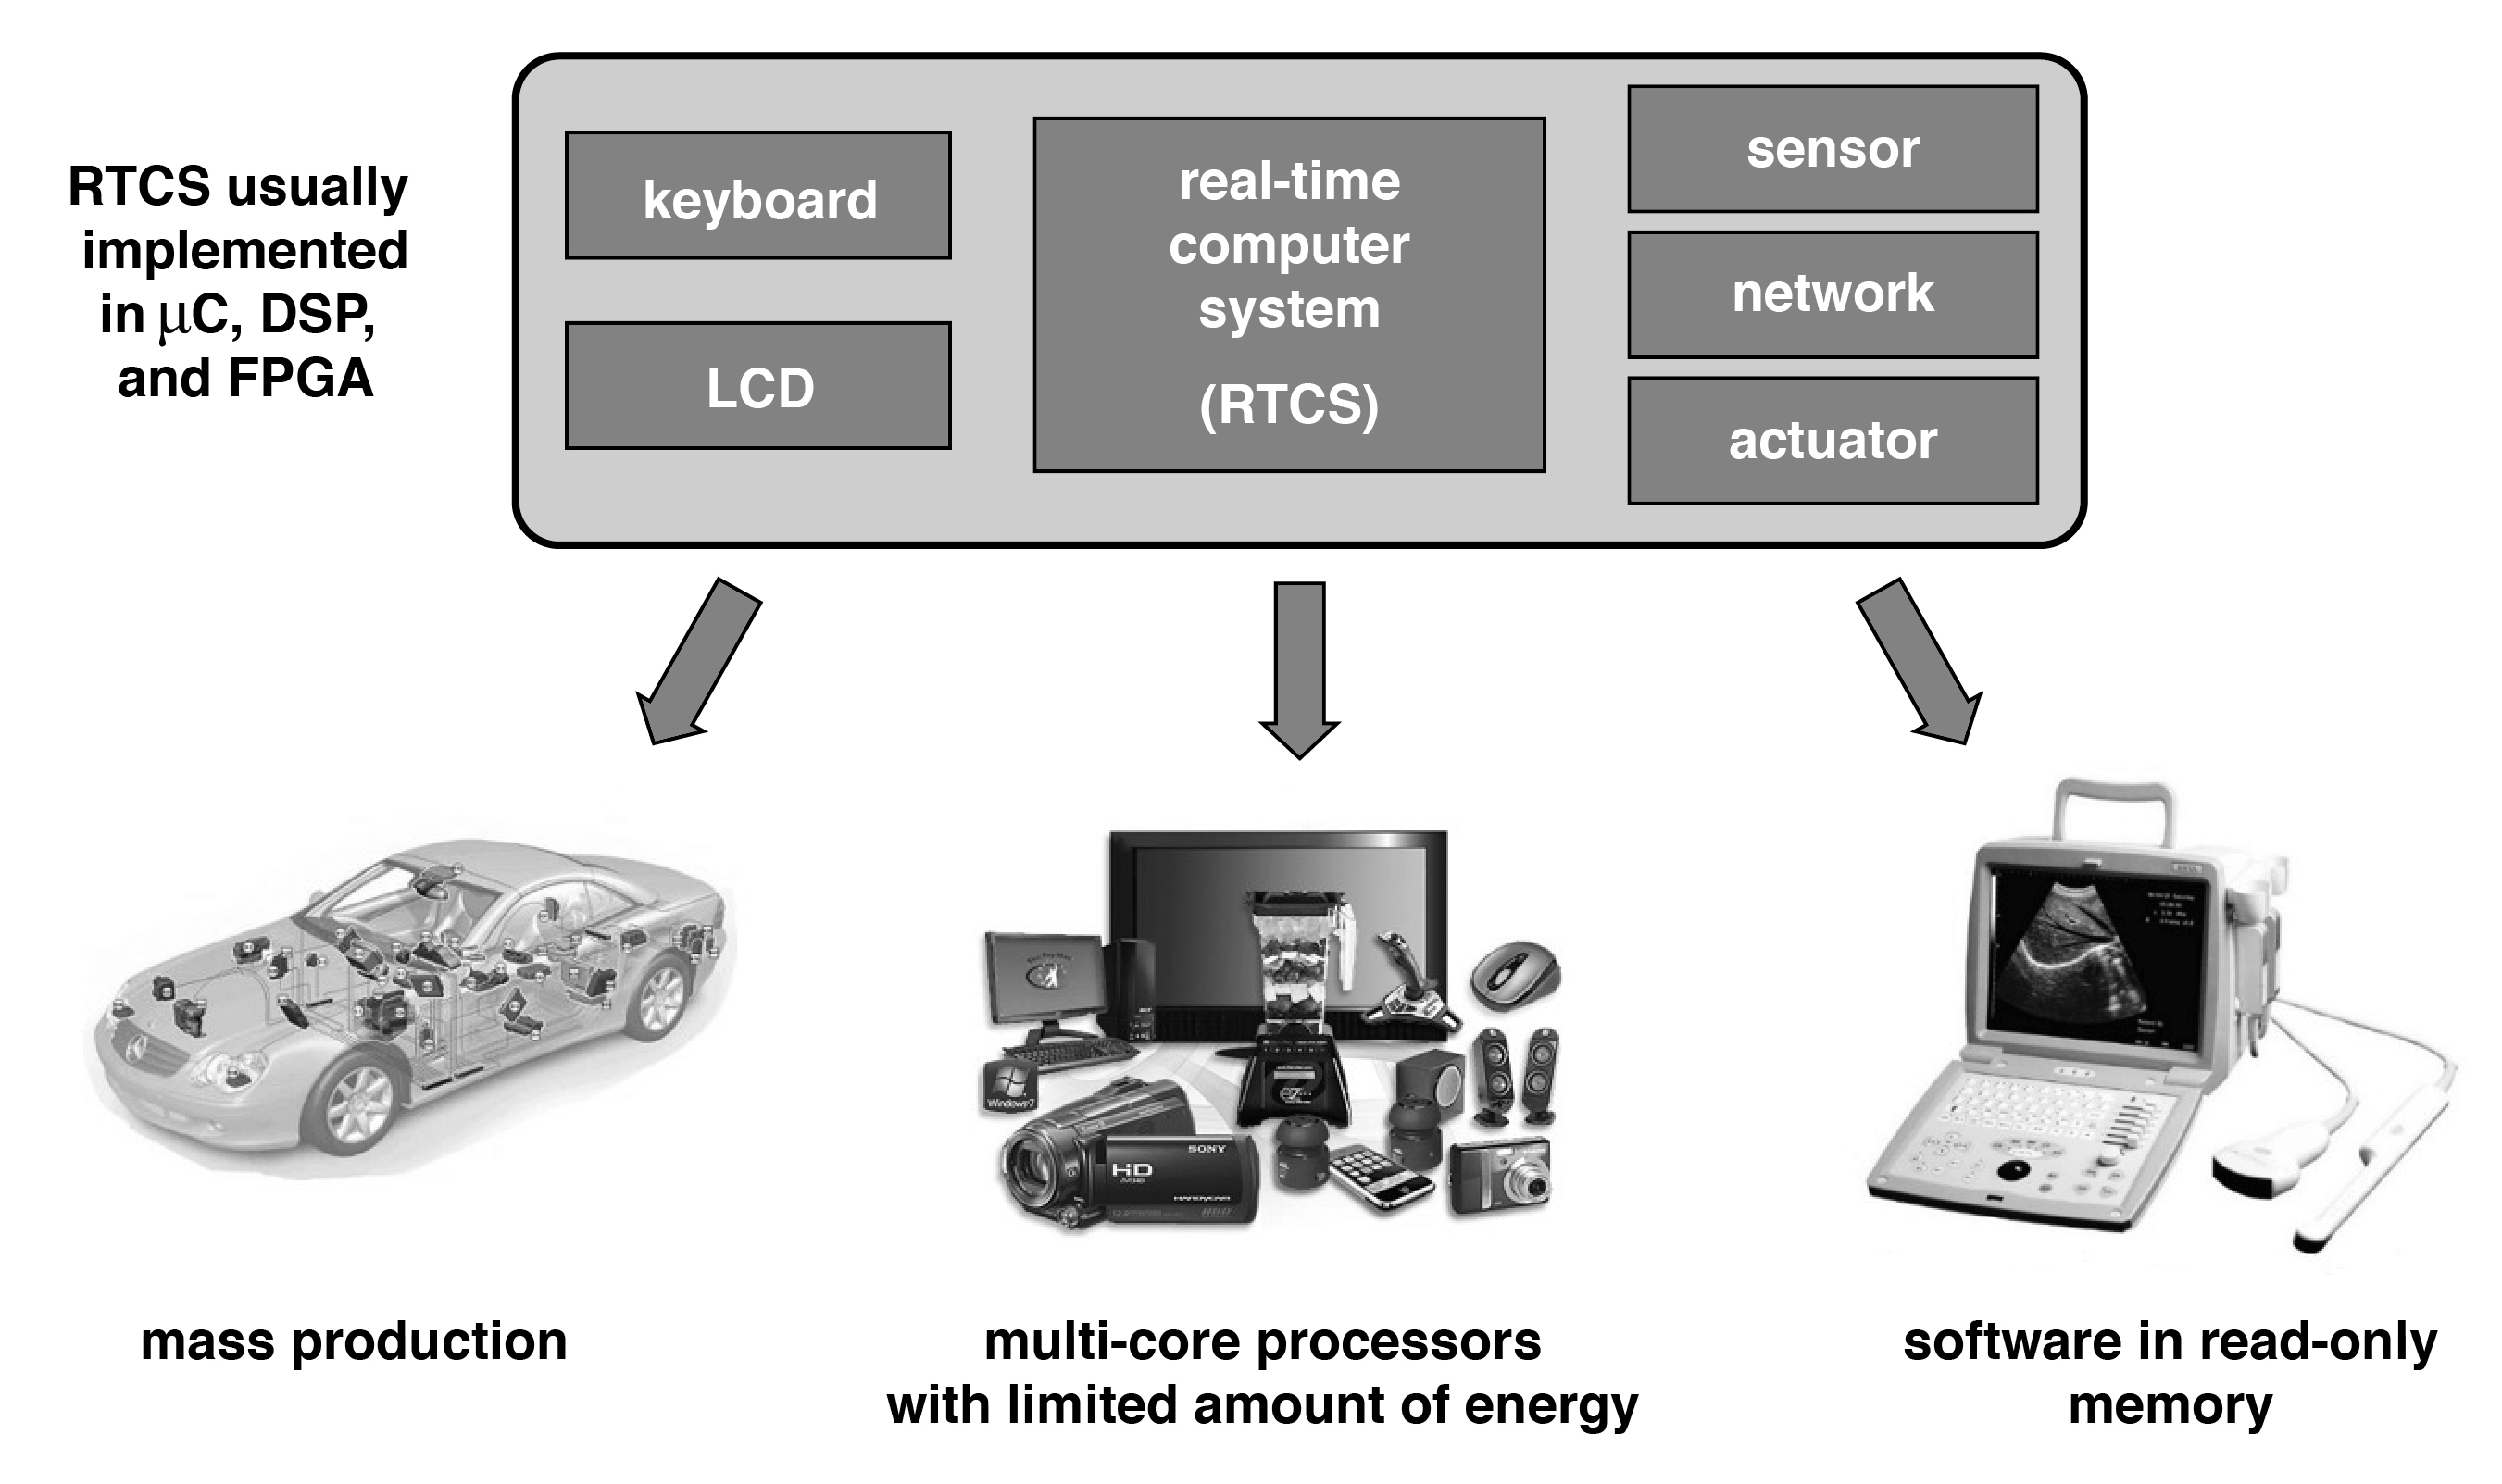
\includegraphics[width=\textwidth]{figure1.jpg}
	\caption{An embedded system is part of a well-specified larger one (intelligent product).}
	\label{intelligent-product}
\end{figure}

Besides, when physical interaction with the real world is needed, which happens in ECPSs, additional care must be taken, mainly when human action is directly replaced, as in vehicle driving. Regarding the latter, even human-in-the-loop feedback control can be employed \cite{munir}, which then raises deeper concerns related to reliability of human behavior modeling and system implementation. Consequently, it is important to go beyond design correctness and also address behavior correctness, which may be performed by incorporating system models. Specifically, such models can be used to evaluate and even synthesize a given particular system, by ensuring that all needed functions are correctly implemented and the correct behavior is exhibited, {\it i.e.}, the system is indeed correct by its method of construction~\cite{Abate17}.

For instance, one may argue that a Linux device driver \cite{ldd} was verified and correctly uses the related kernel services ({\it e.g.,} exported symbols and scheduling); however, not much can be said about correct access to the associated hardware and its use, {\it i.e.}, if \textit{read} and \textit{write} operations are performed according to what is specified in the device's datasheet and setup periods are respected, for instance. In summary, the main goal would be to ensure that the developed driver is compliant with the underlying hardware, which goes further than code correctness and also tackles interaction with surrounding entities.

Regarding behavior correctness, one important observation is that it is becoming more difficult, since fixed mathematical models are being replaced by machine learning approaches (ML) \cite{mlembe}, where future operation may change based on data acquired during previous actions, due to model updating. As a consequence, system-correctness verification procedures should also adapt somehow and incorporate new checks, which may also rely on ML, when analyzing target models or fed with acquired data, as recently reported in the literature~\cite{DBLP:conf/cav/HuangKWW17,DBLP:conf/cav/KatzBDJK17}, where formal verification techniques are applied to verify deep neural networks.

A number of distinctive characteristics might influence the ECPS verification and synthesis process, which include: mass production and static structure, functionality determined by software in read-only memory, multi-core processors with scalable shared memory, and limited amount of energy. Additionally, increasing computational power and decreasing size and cost, which are common to the area of computer processors, are enabling system designers to move more features to software domain, which consequently leads to difficulties in verifying design correctness, since stringent constraints imposed by the underlying hardware ({\it e.g.}, real-time, memory allocation, interrupts, interfacing, and concurrency)~\cite{Kroening15} or even new structures provided with the goal of ensuring more computational capacity~\cite{cudalucas} must be considered during verification. Such observations expand the addressed issues and even complement what was previously mentioned.

The goals of the present article is to briefly present part of the established research and also clarify current trends, which are mainly driven by ECPSs, IoT, and ML. We present a brief discussion about models for ECPSs, in Section \ref{sec:model}, and then cover preliminaries on bounded model checking, \textit{k}-induction verification based on invariant inference, Craig interpolants, counterexample guided inductive synthesis, and system model incorporation, in Section~\ref{Preliminaries}. In Section~\ref{Verification-Challenges}, the main challenges regarding verification and synthesis of embedded systems are described, while Section~\ref{Research-Problem} tackles those challenges that are (partially) open in current published research. Section~\ref{achievements} then describes current achievements and future trends in verification and synthesis of ECPSs and Section \ref{Newapp} addresses new applications, which take into account the new trends ({\it e.g.}, ML) mentioned here. Finally, we conclude and describe future work, in Section~\ref{conclusions}.

%--------------------------------------
\section{Automated Verification and Synthesis of Cyber-physical systems}
\label{sec:model}
%--------------------------------------

Automated formal verification has been employed to ensure correctness and reliability of ECPSs, during the last decade, as well as controller synthesis for ECPSs and HSs \textcolor{red}{add citations}. 

An ECPS $S$ can be represented as a tuple $S=(X,X_{0},U,Y,r,v)$, where $X$ is a set of reachable states, $X_{0}$ is a set of initial states, $U$ is a set of inputs, $Y$ is the set of outputs, $r$ is a transition function such that $r:X\times U \rightarrow X$, and  $v$ is an output mapping function such that $v:X\times U \rightarrow Y$~\cite{Rungger16,Alur00,Girard11}.

The overall automated formal synthesis process for ECPSs and HSs involves three main steps: \textit{modeling}, which is related to obtaining a sound mathematical representation able to capture all relevant aspects of continuous and discrete dynamics and their interaction, as well as formulating properties and invariants that describe a desirable behavior, \textit{verification}, where a ECPS's behavior is checked through the proposed mathematical structure and compliance with a desired behavior is verified, and, finally, controller \textit{synthesis}, which produces a controller or finds invariant control laws that allow a ECPS to meet requirements and behave as desired, which is confirmed by a verification oracle. 


%--------------------------------------
\subsection{A Model for Cyber-physical Systems}
\label{ssec:model}
%--------------------------------------

Models are largely employed in science and engineering areas, in order to analyze, predict, and modify the behavior of real-world systems. Specially, deterministic and stochastic models are the basis of many recent engineering advances. The former is uniquely determined by parameter values and previous states, while the latter presents inherent randomness, which is described by probability distributions~\cite{stochmodel}. Nonetheless, one can argue that such models are not enough to represent ECPSs, since interaction among different entities (software and hardware components) presents several events, which could not be deterministically or stochastically modeled; they should be better represented by nondeterministic approaches~\cite{leeCPS2}. Indeed, that is even more evident when unknown properties are addressed, such as human behavior.

On the one hand, early representations of hybrid systems, {\it i.e.}, systems that mix continuous and discrete dynamics, consisted in instantiating discrete components and discretized continuous dynamics by using discrete models and considering non-modeled effects as uncertainties or perturbations exogenous to them, which can even be negligible. On the other hand, that approach is not suitable for complex ECPSs, which present intense nondeterminism, where uncertainties play a central role and might invalidate the entire system behavior. Indeed, ECPSs have been modeled through different structures that present different degrees of nondeterminism and balance between continuous and discrete dynamics, such as timed automata~\cite{Alur94}, hybrid automata~\cite{Alur93,Henzinger95}, and stochastic hybrid automata~\cite{Julius09,Ghosh05,Pola03}.

Timed automata targets real-time systems and employs finite automata with clocks, {\it i.e.}, real variables that follow continuous trajectories (behaviors) with constant slope. Hybrid automata bridges digital processing and analog entities and consequently generalizes timed automata, by also employing finite automata with real variables, but whose trajectories follow more general dynamical laws~\cite{Henzinger95}.  Timed automata and hybrid automata are deterministic models for hybrid systems that built the basis of HS representations, which were subdivided into different classes of hybrid automata, depending on mapping functions ($r$ and $v$), {\it e.g.}, linear hybrid automata~\cite{Lafferriere99}, rectangular hybrid automata~\cite{Puri94,Henzinger95}, nonlinear hybrid automata~\cite{Henzinger95NL,Broucke1997}, integration graphs~\cite{Kesten1993}, and linear stochastic hybrid automata~\cite{Julius09}. Recently, Rungger and Tabuada~\cite{Rungger16} and Tabuada {\it et al.}~\cite{Tabuada14} proposed a general and wide model for ECPSs, which is based on hybrid automata, by providing the concept of robustness and important tools for robust stability analysis. In addition to HA and TA based models, there are a number of other ECPS modeling initiatives based on (exact or approximate) bisimulation~\cite{Girard11}, simulation~\cite{Rungger13} and interval analysis~\cite{Li16}.



Another approach to ECPS modeling tackles quantized control systems and finite-word length (FWL) effects on the performance of those systems. Differently from bisimulation, quantized models are built from a countable subset of the (quantized) input space~\cite{Tabuada07}. In particular, Keel and Bhattacharyya showed that even robust and optimal controllers may still present an undesired property~\cite{Keel01,bhattacharyya}: fragility or sensitivity to implementation aspects ({\it e.g.}, FWL representations of digital controllers). Therefore, various studies tried link sampled-data theory to hybrid-system models~\cite{Bicchi02,Petreczky10,Petreczky07,Ye98}.

Finally, in addition to ECPS-dynamics modeling, it is often interesting to establish invariants on a ECPS's state space, which can be used for accelerating formal verification and synthesis processes regarding those systems. Such invariants might be synthesized, in order to point out state-space boundaries~\cite{BenSassi12} and determine ECPS stability~\cite{Paul14} or reachability~\cite{Li16_2,Li16}.


%Following their proposal, a CPS $S$ is a tuple $S=(X,X_{0},U,Y,r,t)$, where $X$ is a set of reachable states, $X_{0}$ is a set of initial states, $U$ is a set of inputs, and $r$ is a transition function, such that $r:X\times U \rightarrow X$.



%\textcolor{red}{seria legal falar que nao determinismo pode ser tratado com model checking e ligar com o nosso trabalho... inclusive , o tabuada tem um artigo falando sobre seguranca e SMT, que eu comentei abaixo}




%--------------------------------------
\subsection{Automated and Formal Verification of Cyber-physical systems}
\label{ssec:verification}
%--------------------------------------

Given a class of ECPSs $\Omega$ and a set $\Phi$ of desired properties, a class of verification problems is called decidable if there is an algorithm that is able to decide if a finite number of steps $\forall \mathcal{O}\in\Omega$ satisfy every property $\mathcal{L}\in \Phi$~\cite{Alur00}. Decidability is a key issue in ECPS verification, since there are uncountable states and complex dynamics to be considered, {\it i.e.}, hybrid automata and their variations (usually employed to model ECPSs) are infinite-state machines~\cite{Henzinger95}. In particular, the safety verification of ECPS is undecidable, except in very specific cases as in systems that can be represented by timed automata and rectangular automata~\cite{Alur11}. An alternative to ensure that ECPS trajectories will not pass through unsafe states is the use of barrier certificates~\cite{Prajna07,Prajna04}. An example of barrier certificate is the stability, that ensures the convergence of states to an equilibrium point and consequently that there exists a region from where any trajectory remains inside of this region. The stability may be ensured based on Lyapunov theory (for a wide class of model abstractions)~\cite{tabuada2009verification}, or linear system stability theory for discrete simulations~\cite{Bessa17}. 


Generally, properties that must hold for ECPSs are related to safety/reachability and liveness, and the earliest works on HS and ECPS proposed approaches based on computational tree logic and linear temporal logic~\cite{Alur93}, in order to specify properties and verify those systems. In the last decade, the signal temporal logic~\cite{Maler04,Donze12} was proposed and have been used since then for this purpose, thus providing more suitable operators for dynamic systems and signal processing. Therefore, model-checking procedures have been employed to verify those properties, even under undecidability conditions via approximations, {\it e.g.}, bounding the number of steps from initial states, which leads to bounded model checking (BMC)~\cite{Veanes09}. 

Along with CPS modeling and verification techniques purely based on HA, one can also highlight logic-based approaches~\cite{Phan15} that may still use HA, but are not based on a algebraic description of states and transitions. Some examples of logic-based verification are theorem proving techniques, {\it e.g.} deductive verification (i.e., interactive theorem proving)~\cite{Nipkow02} and automatic theorem proving~\cite{Platzer07}, and reduction-based techniques, among which BMC stands out~\cite{handbook09}.
 

%Much of the work related to the formal verification of ECPS seeks to ensure the safety, robustness, and reachability properties of an HA. 
Recently, some studies have addressed ECPS formal verification considering discretization, switching, and quantization effects.  Dugirala and Viswanathan~\cite{Duggirala2015} verified embedded control software considering real time issues, {\it e.g.}, delayed responses and possible loss of real time deadlines. Anta {\it et al.}~\cite{Anta10} presented a tool called Costan, which finds errors in mathematical-model implementations and verifies whether error is tolerated, considering quantization effects and fixed-point implementation, while focusing on quantization error effects over system stability. Similarly, Ismail {\it et al.}~\cite{dsv_spin2015} preseted DSVerifier, a BMC tool for digital systems that employs SMT/SAT solvers as back-ends, in order to provide support for digital system design and verification considering FWL effects. In particular, DSVerifier checks if a designed digital controller and/or closed-loop ECPS presents the desired performance, when it is implemented with a FWL format~\cite{Bessa16,Bessa17}.

Finally, it is worth mentioning that there are other alternatives for ECPS modeling and analysis, which are not based on verification, but instead on simulators~\cite{Phan2014,Nakajima12,Junjie12}. Although such approaches generally fail in ensuring that some properties hold, they present good scalability, which is ideal for large scale and complex systems that are hardly modeled through automata- or logig-based approaches. Modelica~\cite{Junjie12} and Simulink/MATLAB~\cite{Nakajima12} are important examples of widely used simulators for ECPSs. In order to achieve a balanced trade-off between ECPS-simulation scalability and correctness of verification methods, statistical model checking have been employed to formally verify ECPSs~\cite{Clarke11}.


In addition, Shoukry {\it et al.} \cite{Shoukry} tackled another important problem related to ECPSs: security. Indeed, the essence of ECPSs claims for sophisticated interfacing ({\it e.g.}, sensors and network connections), which normally leads to security issues~\cite{cpsattack}, given that wrong control actions can be generated through corrupted measurements. The mentioned authors proposed a methodology for estimating physical-system state, through formal methods, even if sensor inputs are contaminated with erroneous or intentionally corrupted data, in order to still be able to execute suitable control commands. Cyber-security is also a concern of Fiore {\it et al.}, who aim to ensure secure-state estimation of UAV systems under sparse attacks~\cite{Fiore17}. Indeed, many situations can be regarded as satisfiability problems and solved, for instance, with approaches based on Satisfiability Modulo Theories (SMT)~\cite{Araujo16,TrindadeDAES2016,Rahman13}, which indicates many links with other research areas and might lead to a unified approach regarding system verification, security enforcement, and interaction handling.

%--------------------------------------
\subsection{Control synthesis of Cyber-physical systems}
\label{ssec:synthesis}
%--------------------------------------

Control synthesis for ECPSs consists in finding a controller or an invariant control law $\mathcal{C}$, such that a closed-loop system composed of $(\mathcal{C},\Omega)$ satisfies every property $\mathcal{L}\in \Phi$. 

An efficient way to synthesize reliable ECPSs is Counterexample Guided Inductive Synthesis (CEGIS)~\cite{David15}. Its key idea is the definition (by a user) of a set of safe states, {\it i.e.}, the specification of $\Phi$, as well as a generic template for a control system that must satisfy such a specification. Then, a CEGIS engine compute values for the unknown symbols of the chosen template, which hold $\Phi$~\cite{RienerKFB16}. Abate~{\it et al.}~\cite{Abate17,abatecav2017} presented a method for synthesizing stable controllers that are suitable to continuous plants given as transfer functions~\cite{Abate17} and state-space representations~\cite{abatecav2017}, which exploits bit-accurate verification of software implemented in digital microcontrollers~\cite{Bessa16,Bessa17,dsv_spin2015}, and the resulting systems must ensure non-fragile stability~\cite{Abate17} and safety~\cite{abatecav2017}. Ravanbakhsh and Sankaranarayanan~\cite{Ravanbakhsh15,Ravanbakhsh16} also employed CEGIS based on the Lyapunov's function to ensure the robust reach-while-stay property ({\it i.e.}, a safety specification)~\cite{Ravanbakhsh16} and non-zeno behavior~\cite{Ravanbakhsh15}. CEGIS was also employed to synthesize model predictive controllers for a wide varieties of applications, {\it e.g.} heating ventilation and air conditioning systems, autonomous vehicles control, and aircraft electric power system~\cite{Ghosh05,Rahman13}.

CEGIS is an important, but not the unique, example of symbolic control synthesis for ECPSs. The main advantage of using symbolic synthesis techniques ({\it e.g.}, SMT- and SAT-based) is the possibility of encoding (via logic formulae) reachability/safety specifications on original concrete systems. Indeed, there are many studies~\cite{Rungger13,AydinGol14,Holub16,Tabuada08,Zamani17,Zamani14,Zamani13,Zamani12,Alkhatib17,Lesser15,Girard13} on symbolic control synthesis for ECPS, available in literature.

A common procedure for controller synthesis for ECPS is based on finite-state approximations of infinite-states systems, {\it i.e.}, the HA. Such an approach allows the fully automated synthesis of ECPS control systems that ensure achievement of complex specifications; however, the main weakness of this approach is that it often produces complex controllers with high implementation cost. In order to avoid that problem, refined controllers have been proposed, which aim to provide some invariant properties for close-loop systems, {\it e.g.}: safety~\cite{Dallal17,Dallal13,Girard13}, reachability~\cite{Alkhatib17,Habets06}, stability~\cite{Zamani12,Tabuada08}, and safety/reachability properties, considering quantization effects~\cite{Reissig17}.


% The mentioned authors developed a tool called DSSynth, which is able to synthesize digital controllers that are algorithmically and numerically sound, w.r.t. stability. DSSynth marks the first use of counterexample-guided inductive synthesis~\cite{sketch} to synthesize digital controllers, considering physical plants with uncertain models and FWL effects; however, low-level implementation errors ({\it e.g.}, limit cycles) are not further investigated.

%--------------------------------------
\section{Bounded Model Checking (BMC)}
\label{Preliminaries}
%--------------------------------------

Bounded Model Checking (BMC) based on Boolean Satisfiability (SAT) was originally proposed to verify hardware designs~\cite{Biere99,handbook09}. Indeed, Biere {\it et al.} were able to successfully verify large digital circuits with approximately $9510$ latches and $9499$ inputs, leading to BMC formulae with $4 \times 10^6$ variables and $1.2 \times 10^7$ clauses to be checked by standard SAT solvers. BMC based on SMT~\cite{BarrettSST09}, in turn, was originally proposed to deal with increasing software verification complexity~\cite{Armando2009}. 
%
In general, BMC techniques aim to check the violation of a given (safety) property at a given system depth, as shown in Figure~\ref{bounded-model-checking}. 
%
\begin{figure}[h]
	\centering
	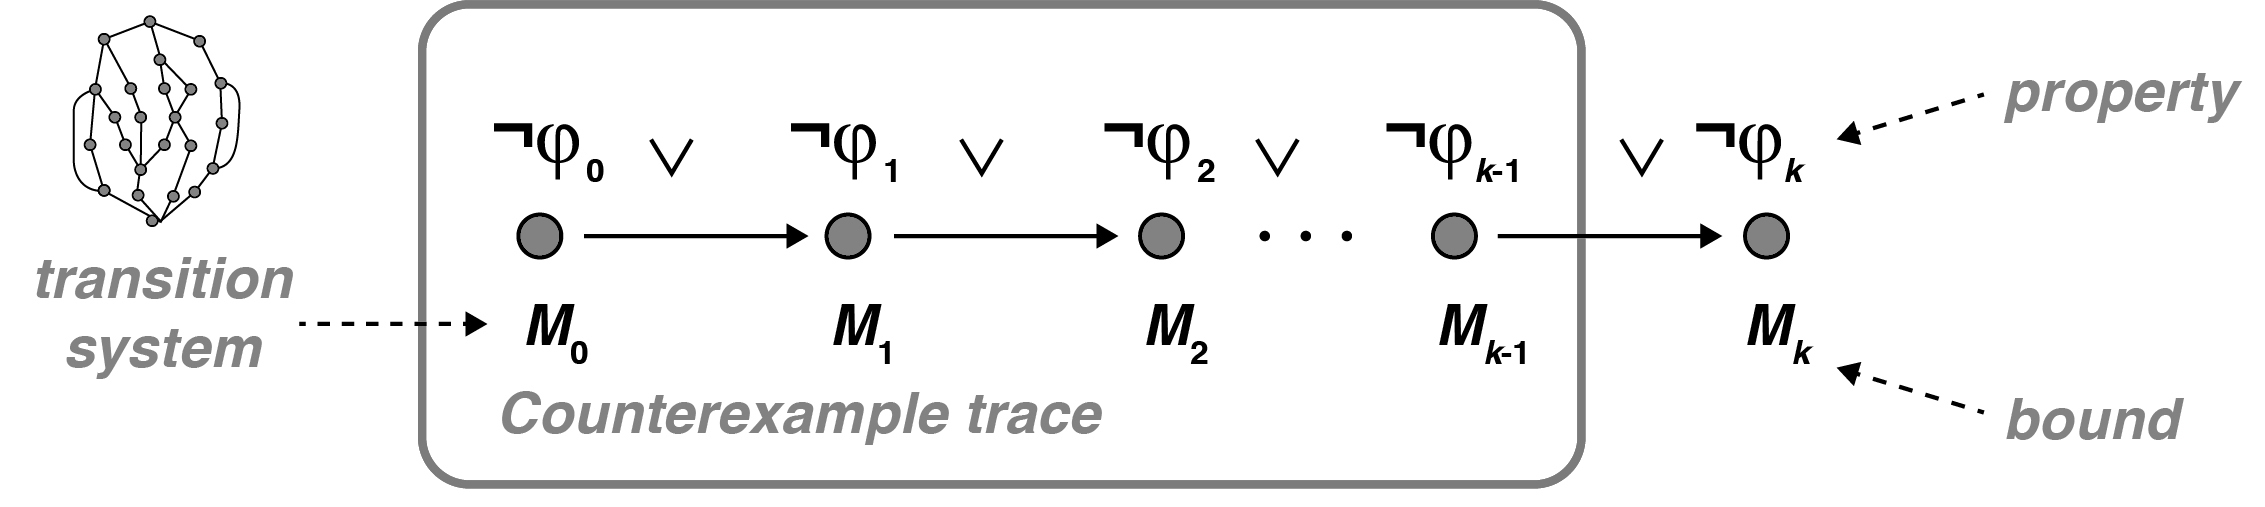
\includegraphics[width=\textwidth]{figure2.jpg}
	\caption{Bounded Model Checking.}
	\label{bounded-model-checking}
\end{figure}

Indeed, given a transition system \textit{M}, which is derived from the control-flow graph of a program, a property $\phi$, which represents program correctness and/or a system's behavior, and an iteration bound \textit{k}, which limits loop unrolling, data structures, and context-switches, BMC techniques thus unfold a system \textit{k} times, in order to convert it into a verification condition $\psi$, which is expressed in propositional logic or in a decidable-fragment of first-order logic, such that $\psi$ is \textit{satisfiable} if and only if $\phi$ has a counterexample of depth less than or equal to \textit{k}. The propositional problem associated with SAT-based BMC is formulated by constructing the following equation~\cite{Biere99}:
%
\begin{equation}
\label{bounded-model-checking-biere}
\psi_{k} = I\left(s_{0}\right) \wedge \bigwedge^{k-1}_{i=0} R\left(s_{i},s_{i+1}\right) \wedge \neg \phi_{k}
\end{equation}

\noindent Here, $\phi_{k}$ represents a safety property $\phi$ in step $k$, $I$ is the set of initial states of $M$, $R\left(s_{i},s_{i+1}\right)$ is the transition relation of $M$ at time steps $i$ and $i+1$. Hence, the equation $\bigwedge^{k-1}_{i=0} R\left(s_{i},s_{i+1}\right)$ represents the set of all executions of $M$ of length $k$. $\neg \phi_{k}$ represents the condition that $\phi$ is violated in state $k$, which is reached by a bounded execution of $M$ of length $k$. Finally, the resulting (bit-vector) equation is translated to conjunctive normal form in linear time and passed to a SAT solver for checking satisfiability. Eq.~(\ref{bounded-model-checking-biere}) can be used to check safety properties~\cite{PrasadBG05}. Liveness properties ({\it e.g.}, starvation, deadlock) that contain the Linear-time Temporal Logic (LTL) operator $F$ are checked by encoding $\neg \phi_{k}$ in a loop within a bounded execution of length at most $k$, such that $\phi$ is violated on each state in the loop. In this case, Eq.~\ref{bounded-model-checking-biere} can be rewritten as:

%
\begin{equation}
\psi_{k} = I\left(s_{0}\right) \wedge \bigwedge^{k-1}_{i=0} R\left(s_{i},s_{i+1}\right) \wedge \left(\bigvee^{k}_{i=0} \neg \phi_{i}\right)
\end{equation}

\noindent where $\phi_{i}$ is the propositional variable $\phi$ at time step $i$. Thus, this equation can be satisfied if and only if for some $i$ ($i \leq k$) there exists a reachable state at time step $i$ in which $\phi$ is violated. 

One may notice that BMC analyzes only bounded program runs, but generates verification conditions (VCs) that reflect the exact path in which a statement is executed, the context in which a given function is called, and the bit-accurate representation of expressions. A verification condition is a logical formula (constructed from the bounded program and desired correctness properties) whose validity implies that the program's behaviour agrees with its specification~\cite{Bradley07}. Correctness properties in programs can be specified by the user via \textit{assert} statements or automatically generated from a specification language~\cite{Thomas01}. If all of a bounded program's VCs are valid, then a program is in compliance with its specification up to the given bound.

As an example, consider a simple C program (slightly modified from~\cite{Strichman08}) with an exponential number of paths, as shown in Figure~\ref{figure:verification-condition}(a); the corresponding C program, in single static assignment (SSA) form~\cite{Appel97}, is shown in Figure~\ref{figure:verification-condition}(b). The SSA form is an intermediate representation, which is used by compilers to facilitate optimizations and transformations of source code. The common property in SSA form is that every variable has only one definition in the program text. This is achieved by introducing a fresh variable from the original name ({\it e.g.}, with a subscript), such that every assignment has a unique left-hand side, as shown in Figure~\ref{figure:verification-condition}(b).
%
\begin{figure}[ht]
\centering
\begin{minipage}{0.45\textwidth}
\begin{lstlisting}
#include <assert.h>
int x[N], a;
...
int main(void) {
  a=N;
  for(int i=0; i<N; i++)
    if (x[i]>1)
      a--;
  assert(a<=N);
  return 0;
}
\end{lstlisting}
\end{minipage}
\begin{center}
(a)
\end{center}
\centering
\begin{minipage}{0.45\textwidth}
\begin{lstlisting}
a1 = N
a2 = (x[0] > 1) ? a1 - 1 : a1
a3 = (x[1] > 1) ? a2 - 1 : a2
a4 = (x[2] > 1) ? a3 - 1 : a3
...
an+1 = (x[N-1] > 1) ? an - 1 : an 
\end{lstlisting}
\end{minipage}
\begin{center}
(b)
\end{center}
\caption{(a) A simple C program with a loop \textit{for}. (b) The corresponding unwound C program of (a) converted into SSA form.} 
\label{figure:verification-condition}
\end{figure}

Apart from that, this program has an exponential number of paths, since each element of $x$ can be either greater than one or less than or equal to one. Despite the large number of paths through that program, BMC unwinds it up to a bound $k$ and translates it into a VC $\psi$, such that $\psi$ is satisfiable if and only if the assertion $a<=N$ fails. One may also notice that BMC still encodes program stages with a size that grows linearly with $N$. More precisely, the program in Figure~\ref{figure:verification-condition}(a) is converted into $\psi$ using a decidable fragment of first-order logic, as follows~\cite{Bradley07}:
%
\begin{equation}              
\label{verification-condition-example}
\psi := \left [ \begin{array}{ll} 
                a_{1} = N  \\
                \wedge \, \, a_{2} = ite\left(x[0] > 1, a_{1} - 1, a_{1}\right) \\ 
                \wedge \, \, a_{3} = ite\left(x[1] > 1, a_{2} - 1, a_{2}\right) \\
                \wedge \, \, a_{4} = ite\left(x[2] > 1, a_{3} - 1, a_{3}\right) \\
                \wedge \ldots \\
                \wedge \, \, a_{N+1} = ite\left(x[N-1] > 1, a_{N} - 1 , a_{N}\right) \\
                \wedge \neg \left(a_{N+1} \leq N\right) \\
              \end{array} \right ]  \\
              \\           
\end{equation}

The ternary operator $f \: \: ? \: \: t_1 : t_2$, shown in Figure~\ref{figure:verification-condition}(b), is converted into the conditional expression $\mathit{ite}(f, t_1, t_2)$ that takes as its first argument the Boolean formula $f$ and, depending on its value, selects either the second (i.e., $t_1$) or the third argument (i.e., $t_2$). In order to verify that the assertion $a<=N$ holds, its negation is added to $\psi$ and it is checked whether the entire formula is satisfiable, through an off-the-self SMT solver. Formula (\ref{verification-condition-example}) can be represented simply as a Boolean logic circuit, which can be further transformed into a (equisatisfiable) conjunctive-normal-form formula over propositional variables, by Tseitin's transform~\cite{Tseitin83} in linear time and by introducing at most a linear number of fresh variables; however, checking the validity of a first-order logic formula, in a given background theory, is an ${\mathcal{NP}}$-complete problem~\cite{PatarinG97}).

From the practical point of view, SAT- or SMT-based BMC procedures have been successfully applied to verify a large number of hardware and software systems, including digital circuits and single- and multi-threaded programs. Those BMC techniques were able to find subtle bugs in real digital and embedded software systems, as reported in the available literature~\cite{Clarke04,MerzFS12,CordeiroF11,Ivancic05,Cordeiro12}. Nonetheless, the main criticism with respect to BMC techniques relies on completeness, since they are able to prove system correctness only if an upper bound \textit{k} is known, {\it i.e.}, a bound that unfolds all loops and recursive functions to their maximum possible depth. 

Due to that limitation, BMC tools are typically susceptible to exhaustion of time or memory limits, when checking complex circuit-implementations or programs with loops, whose bounds are too large or cannot be statically determined. Indeed, such an issue has pushed researchers to overcome the depth limitation and propose extensions capable of proving global correctness.

%--------------------------------------
\subsection{Induction-based Verification of C Programs}
%--------------------------------------

One promising approach to achieve completeness, in BMC techniques, is to prove that an invariant (assertion) is \textit{k}-inductive~\cite{EenS03,Sheera00}; however, the main challenge regarding such an approach relies on computing and strengthening inductive invariants from programs. In particular, loop invariants, which are computed from programs under verification, must be inductive (and not just invariant), in order to check the corresponding VCs, {\it i.e.}, induction cannot determine invariance of a non-inductive assertion~\cite{Bradley07}. 

For instance, consider the C-code fragment shown in Figure~\ref{figure:inductive-invariant}. If we consider the IEEE floating-point standard (IEEE 754)~\cite{4610935,Goldberg91whatevery}, then  the loop invariant $x>0$ holds initially and after each iteration; actually, $x$ tends to infinity after $128$ iterations. Nonetheless, this invariant is not inductive, given that $x>0$ before an initial iteration does not ensure that $x>0$ after each iteration; if we initially have $x=0.9$, then $x<0$ after the fourth iteration. As a consequence, even if invariant generation procedures successfully compute such assertions, which are indeed invariant, those must be inductive, so that \textit{k}-induction verifiers can automatically prove program correctness. In this specific example, an inductive invariant would be $x>1$, given that if we can check that if $x>1$ before the initial iteration, then also $x>1$ after \textit{k} iterations.
%
\begin{figure}[h]
\centering
\begin{minipage}{0.45\textwidth}
\begin{lstlisting}
#include <assert.h>
int main(void) {
 float x=2;
 while (1) {
   x = ((2*x) - 1);
 }
 return 0;
}
\end{lstlisting}
\end{minipage}
\caption{Motivating example for inductive invariants.}
\label{figure:inductive-invariant}
\end{figure}


There are several invariant-generation algorithms that discover linear and polynomial relations among integer and real variables, in order to provide loop invariants and also discover the memory ``shape'', in programming languages with pointers~\cite{pips:2013,Henry:2012}. The current literature also reports successful applications of \textit{k}-induction based verification algorithms for hardware and software systems, using invariant generation and strengthening, mostly based on interval analysis~\cite{Beyer15}. 

Novel verification algorithms for proving correctness of (a large set of) C programs, by mathematical induction and in a completely automatic way ({\it i.e.}, users do not need to provide loop invariants), were recently proposed~\cite{Gadelha15,Beyer15,Brain15,Rocha15,Kinductor,Rocha17}. Additionally, \textit{k}-induction based verification was also applied to ensure that (restricted) C programs (1) do not contain violations related to data races~\cite{Donaldson10}, considering the Cell BE processor, and (2) do respect time constraints, which are specified during system design phases~\cite{EenS03}. Apart from that, \textit{k}-induction is also a well-established technique in hardware verification, where it is easily applied, due to the monolithic transition relation present in such designs~\cite{EenS03,Sheera00,GrosseLD09}.

It is worth noticing that \textit{k}-induction with invariants has the potential to be directly integrated into existing BMC approaches, given that the induction algorithm itself can be seen as an extension after \textit{k} unwindings and it is possible to generate program invariants with other software modules, which are then translated and instrumented into an input program \cite{Rocha15}.

Nonetheless, there is~little evidence, in the available literature, that model checking hardware and software systems through \textit{k}-induction (and invariants) can be efficiently exploited in ECPS verification. That happens due to the distinctive characteristics mentioned earlier, which influence ECPS development and also verification processes. Additionally, there is still a lack of studies for embedded software verifiers to exploit the combination and configuration of different invariant generation and strengthening algorithms, including analysis to discover linear inequalities, polynomial equalities and inequalities, and invariants related to memory and variable aliasing~\cite{Bradley07}.

%------------------------------------------------------
\subsection{Craig Interpolation}
\label{sec:CraigInterpolationInModelChecking}
%------------------------------------------------------

Another feasible alternative to prove properties in BMC is to compute Craig interpolants for inconsistent pairs (or more generally, sets) of formulae~\cite{McMillan03,McMillan05,McMillan06,McMillan07}. This alternative approach exploits the SAT/SMT solvers' ability to produce refutations, {\it i.e.}, proofs regarding the nonexistence of counterexamples of depth less than or equal to $k$. Those proofs do not ensure whether a given property holds in the model, but they contain information about reachable states of a model.

%\begin{prf}\label{interpolants}
\begin{definition}\label{interpolants}
\textit{Given a pair of formulae $\left(A,B\right)$, such that $A \wedge B$ is inconsistent, and a proof by resolution for $\left(A,B\right)$, an \textit{interpolant} for $\left(A,B\right)$ is a formula $F$ with the following properties~\cite{McMillan03,McMillan05}: }

\begin{itemize}
	\item $A \Rightarrow F$;
	\item $F \wedge B$ \textit{is unsatisfiable};
	\item $F$ \textit{expressed only over the common variables (nonlogical symbols) of $A$ and $B$}.
\end{itemize}
\end{definition}
%\end{prf}

As an example, consider $A = \left(x_1 \wedge x_2\right)$ and $B = \left(\neg x_2 \wedge x_3\right)$. Given that $\left(x_1 \wedge x_2\right)$ must imply $F$ (or simply that $\neg x_1 \vee \neg x_2 \vee F$ hold) and $F \wedge \neg x_2 \wedge x_3$ must be unsatisfiable, one possible interpolant for the given pair of formulae $\left(A,B\right)$ is $F = x_2$, since $x_2$ is a common part of both $A$ and $B$. 

The use of interpolants allows us to define a complete method for finite-state reachability analysis based on SAT and SMT solvers. In order to show how BMC and interpolation can be combined, we refer to Section~\ref{Preliminaries} where we define Eq.~(\ref{bounded-model-checking-biere}) and the terms $I$, $R$, and $\phi$. Now, suppose that $Q=I$ and Eq.~(\ref{bounded-model-checking-biere}) is partitioned, so that the set of initial states $I$ and the first instance of the transition relation $R$ are in set $A$, while the remaining instances of $R$ and the property $\phi$ are in set $B$, as shown in Figure~\ref{figure:computing-image-by-interpolation} (note that $k$ is unknown).

\begin{figure}[ht]
\centering
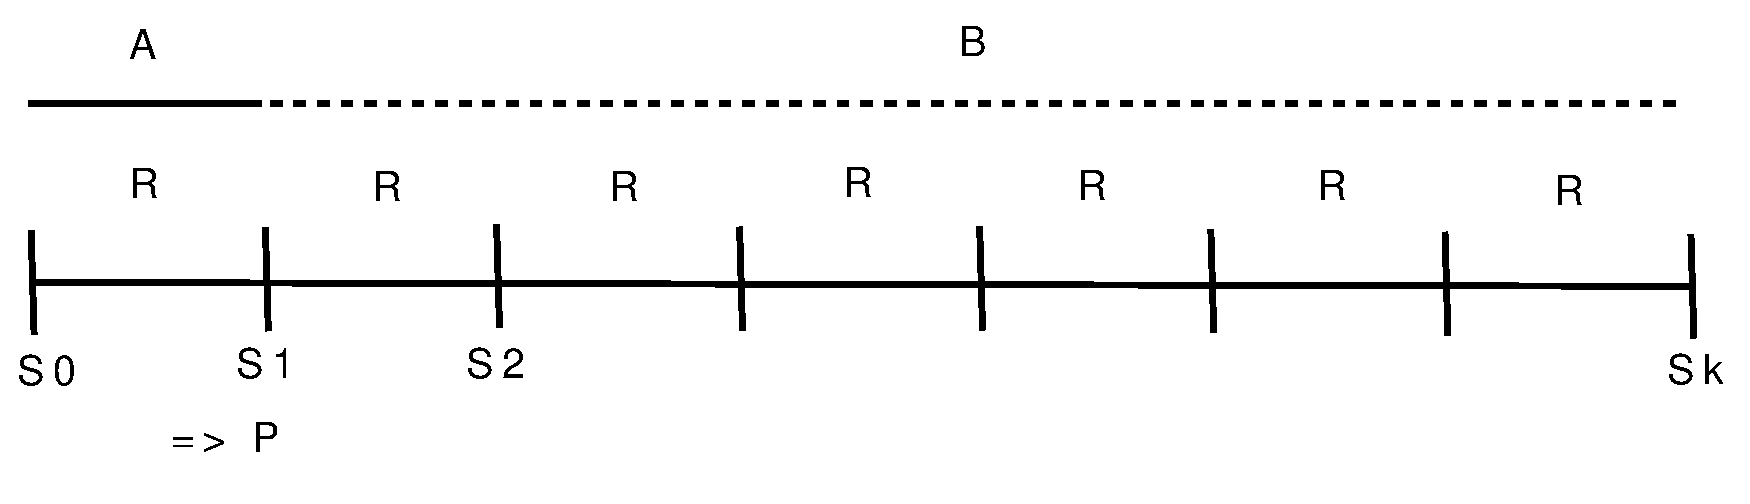
\includegraphics[width=\textwidth]{interpolants}
\caption{Computing image by interpolation~\cite{McMillan03}.}
\label{figure:computing-image-by-interpolation}
\end{figure}


Suppose that we use an SMT solver to prove that the $A \wedge B$ is unsatisfiable, {\it i.e.}, we use an SMT solver to conclude that there is no satisfying assignment to $A \wedge B$.\footnote{Note that if at any stage we can satisfy the property $\phi$ within $k$ steps from the initial state, then we have found a counterexample.} The internal steps performed by the SMT solvers for reaching this conclusion can be used to construct a proof of unsatisfiability $\Pi$. From this proof, we can derive an interpolant $F$ for the pair of formulae $\left(A,B\right)$, i.e., $F = interpolant\left(\Pi, A, B\right)$. According to Definition~\ref{interpolants}, $A$ must imply $F$ and since we defined $A$ to be the set of initial states and the first instance of $R$ (i.e., from Figure~\ref{figure:computing-image-by-interpolation}, $A=s_{0} \wedge s_{1}$), it follows that $F$ is \textit{true} in every state reachable from the initial state in one step. In other words, we can say that $F$ is an over-approximation of the forward image of $I$~\cite{McMillan03,McMillan05}. Also according to Definition~\ref{interpolants}, the formula $F \wedge B$ must be unsatisfiable (from Figure~\ref{figure:computing-image-by-interpolation}, $B=s_{2} \wedge s_{3} \wedge \ldots \wedge s_{k}$), which means that there is no state satisfying $F$ that can reach a final state $s_k$. After computing $F$, we then check whether $F$ implies $Q$. If $F$ implies $Q$, then no reachable state can satisfy the property $\phi$ and we can thus conclude that the property holds; however, since $F$ is an approximation, we can falsely conclude that the final state is reachable. In this case, we update $Q = F \vee Q$ and $A = F \wedge R_{0}$, increase the value of $k+1$ and check whether $A \wedge B$ is unsatisfiable. If $A \wedge B$ is satisfiable, we have found a valid counter-example (i.e., a path from the initial state to the final state); otherwise, we compute the interpolant $F = interpolant\left(\Pi, A, B\right)$ again and check whether $F$ implies $Q$. This procedure is stopped when we have found a valid counterexample or have proved that the final state is not reachable (i.e., the property holds). The details of the algorithm and further information about the use of interpolants in model checking can be found in~\cite{McMillan03,McMillan05,McMillan06,McMillan07}. 

%--------------------------------------
\subsection{Program Synthesis via Counter-Example \\ Guided Inductive Synthesis (CEGIS)}
%--------------------------------------

The basic idea of program synthesis is to automatically construct a program $P$ that satisfies a correctness specification $\sigma$. In particular, program synthesis is automatically performed by engines that use a correctness specification $\sigma$, as starting point, and then incrementally produce a sequence of candidate solutions that satisfy $\sigma$~\cite{Abate17}. As a result, a given candidate program $p$ is iteratively refined, in order to match the specification $\sigma$ more closely. Counter-Example Guided Inductive Synthesis (CEGIS) represents one of the most popular approaches to program synthesis that are currently used in practice~\cite{David15}. Figure~\ref{Counter-Example-Guided-Inductive-Synthesis} shows the basic architecture of the CEGIS approach, which has close connections to algorithmic debugging using counterexamples and abstraction refinement~\cite{Alur13}. 

The correctness specification $\sigma$ provided to the program synthesizer is of the form $\exists \vec{F} .  \forall \vec{x}.  \sigma(\vec{x}, \vec{F})$, where $\vec{F}$ ranges over functions, $\vec{x}$ ranges over ground terms, and $\sigma$ is a quantifier-free formula typically supported by SMT solvers. The ground terms are interpreted over some finite domain $\mathcal{D}$, where $\mathcal{D}$ can be encoded using the SMT's bit-vectors part. The phases {\sc Synthesize} and {\sc Verify} interact via a finite set of test vectors {\sc inputs} that is incrementally updated. Given the correctness specification $\sigma$, the {\sc Synthesize} procedure tries to find an existential witness $\vec{F}$ satisfying the specification $\sigma(\vec{x}, \vec{F})$, for all $\vec{x}$ in {\sc inputs} (as opposed to all $\vec{x} \in \mathcal{D}$). If {\sc synthesize} succeeds in finding a witness~$\vec{F}$, this witness is a candidate solution to the full synthesis formula, which is passed to the phase {\sc verify}, in order to check whether it is a full solution ({\it i.e.}, $\vec{F}$ satisfies the specification $\sigma(\vec{x}, \vec{F})$ for all $\vec{x}\in\mathcal{D}$). If this is the case, then the algorithm terminates; otherwise, additional information is provided to the phase {\sc synthesize}, in the form of a new counterexample that is added to the {\sc inputs} set and the loop iterates again. 
%
\begin{figure}[h]
	\centering
	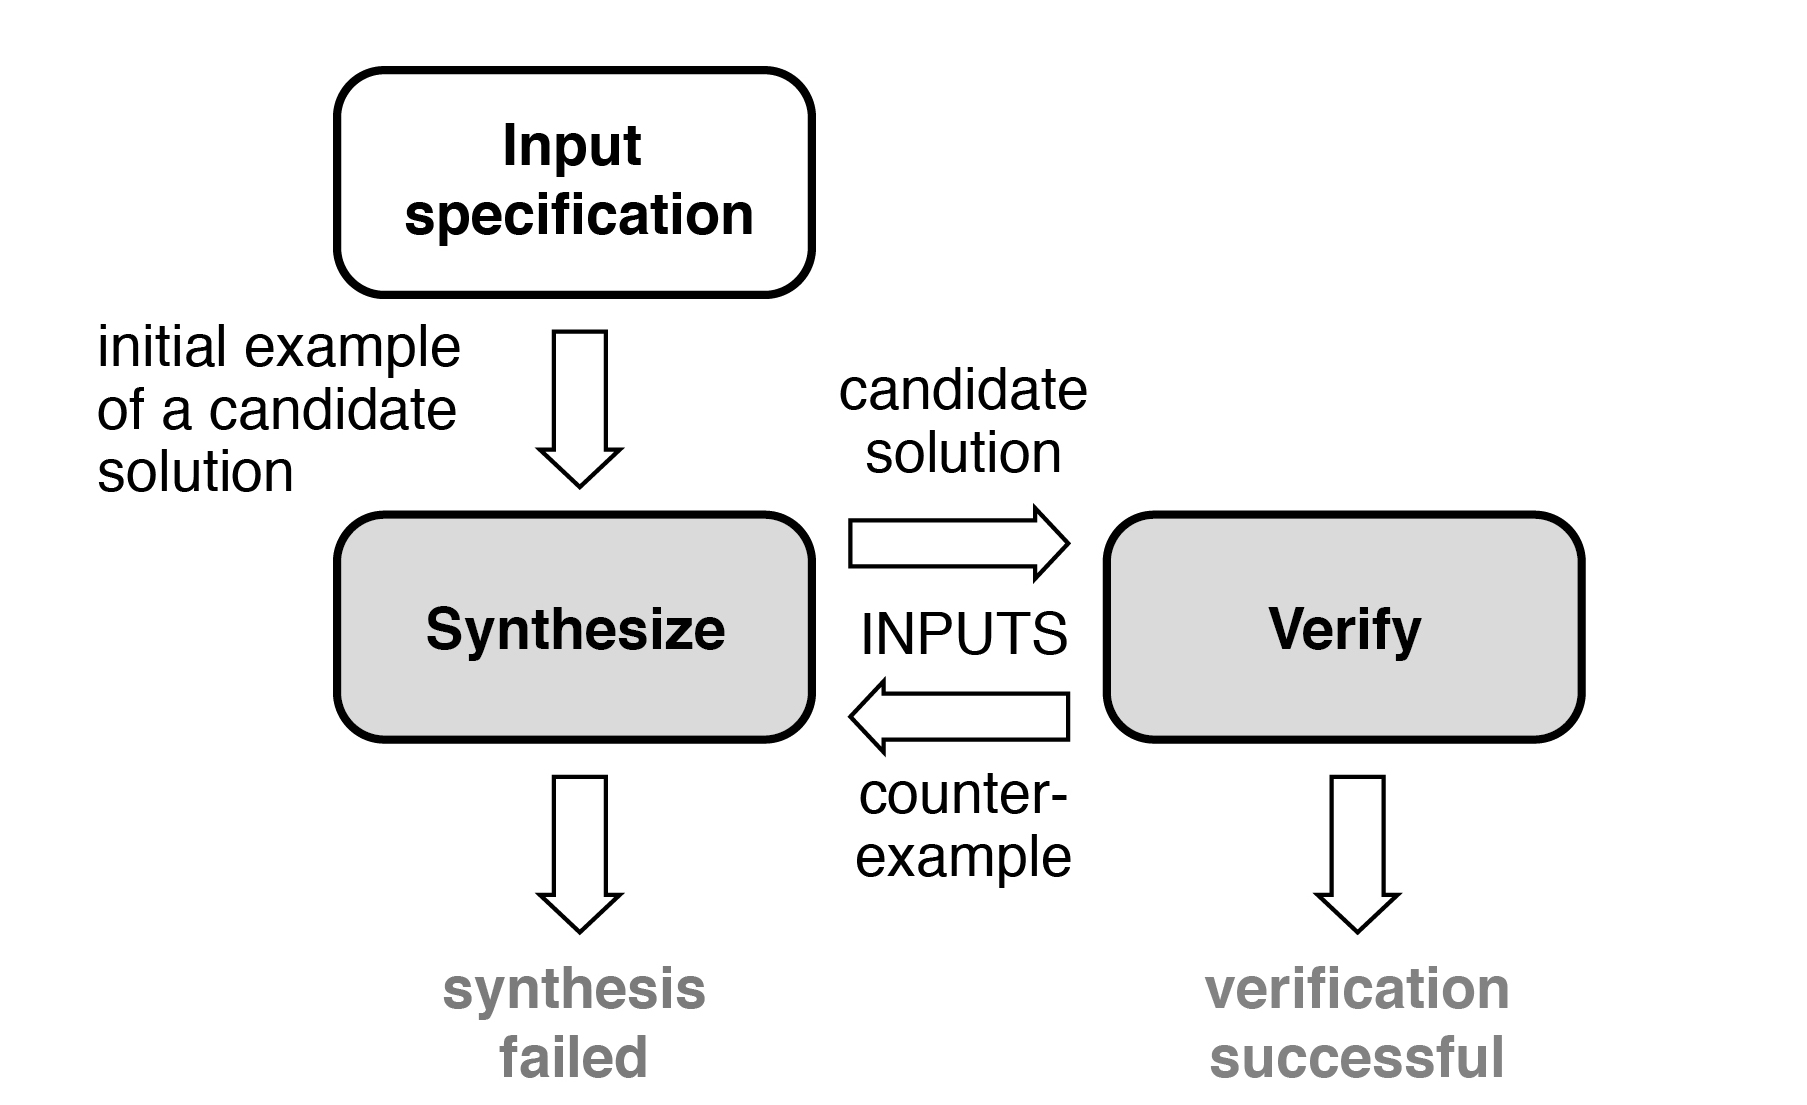
\includegraphics[width=\textwidth]{figure3.jpg}
	\caption{CounterExample Guided Inductive Synthesis (CEGIS).}
	\label{Counter-Example-Guided-Inductive-Synthesis}
\end{figure}

One may notice that each iteration of the CEGIS loop adds a new input to the finite set $\text{\sc inputs}$ that is used for synthesis.  Given that the full set of inputs $\mathcal{D}$ is finite, this means that the refinement loop can only iterate a finite number of times; however, $\mathcal{D}$ can represent a large number of elements for the finite set $\text{\sc inputs}$. In order to avoid exploring all possible values, machine learning techniques can be used in the phase {\sc Synthesize}, with the goal of learning from experience, {\it i.e.}, learning from counterexamples provided by a verification oracle~\cite{Alur13}.

Nowadays, program synthesis engines that implement the CEGIS approach~\cite{sketch} can automatically produce solutions for a large variety of specifications, due to the combination of automated testing, genetic algorithms, and SMT-based automated reasoning~\cite{Sharma14}.

%--------------------------------------
\subsection{Incorporating System Models to Automated \\ Verification and Synthesis Procedures}
%--------------------------------------

Currently, SMT-based BMC approaches check code properties in real programs, which basically address programing-language issues and general correctness, without taking into account target applications or system behavior. Such a statement is important, since, as already mentioned, many system features are being moved to software domain, which then requires schemes that do not only check if source code is correctly written, but also if it will properly respond in real environments or under external problems or corrupted data. For instance, the anti-lock braking system software of a vehicle model can be bug free, but it may not work correctly if a sensor is damaged or even intentionally tampered \cite{Shoukry}.

Indeed, research in software verification is now incorporating such considerations, during checking processes, and some schemes already use knowledge about the system to be verified and the underlying hardware. Recently, a verification tool for digital systems was proposed, which is called digital system verifier (DSVerifier)~\cite{dsv_spin2015,Monteiro16} and is able to aid engineers to check overflow, limit cycle, output error, timing, stability, and minimum phase, considering finite word-length (FWL) effects. Additionally, DSVerifier checks closed-loop systems with uncertain models considering FWL effects, which are typically represented as hybrid systems, {\it i.e.}, the controller is digital but the controlled agent (plant) is a physical and continuous system~\cite{Bessa17}. That ultimately leads to the use of analog-to-digital converters, which are one of the most important aspects to be considered, given that data loss (quantization) is inevitable. As a consequence, verification procedures have to consider the interaction between a continuous plant and a digital (and sampled) controller with FWL effects, which can be connected using different control system configurations. Additionally, the latter may present a different behavior, regarding what was specified in analog domain, due to the inherent discret-time operation. 


In summary, DSVerifier is a useful test tool, which takes into account different representations ({\it e.g.}, transfer-function and state-space), realization forms ({\it e.g.}, direct, delta, and transposed forms), and other implementation restrictions, in order to explore the design space. Finally, if a system's requirements are not met with a given configuration, an analysis of the provided error report may suggest another setup, which can even be incorporated into a given system development procedure, by providing both system verification and model refinement. 

In this respect, DSVerifier has been extended to automatically synthesize digital stabilizing controllers for continuous plants~\cite{Abate17}. In particular, a CEGIS-based approach, implemented in a tool called digital system synthesizer (DSSynth), uses inductive synthesis in conjunction with the DSVerifier's algorithm for verifying robust closed-loop stability that addresses plant variations as interval sets, as well as FWL uncertainties in digital controllers. DSSynth is able to successfully synthesize stable digital controllers for a set of intricate plant models, taken from the control literature, within minutes. Nonetheless, system correction is of paramount importance and, even with such a synthesizing tool, a final verification procedure should be executed, with the goal of ensuring that the generated solution still complies with the provided specs and other issues, which may have not been initial tackled and have the potential to compromise system reliability, are not present.

Apart from the control system domain, Scratch is another example software model-checking tool, which uses knowledge about the system to be verified and the underlying hardware, with the goal of detecting races related to direct memory access (DMA), in the Cell BE processor~\cite{Donaldson10}. That tool also uses BMC, in order to detect DMA races, and BMC with \textit{k}-induction, which aims to prove the absence of races. If support to other DMA operations were added, Scratch could be adapted to different architectures, {\it i.e.}, the same techniques would be employed, but with a different system behavior/knowledge.

One may also notice that such a paradigm, {\it i.e.}, verification and synthesis based on an expected system behavior, is not restricted to digital filters and controllers or DMA races, but it can also be applied to possibly any real system, as long as the desired behavior can be expressed as properties in BMC frameworks. For instance, regarding self-driving cars, an important property could be the detection of pedestrians, animals, bicycles, or any obstacle present on urban and rural roads. Indeed, bicycles are considered one of the most difficult problems, due to the myriad of possible shape and colors \cite{selfcar}. In addition, the mentioned problem is closely related to machine learning, from which refinement strategies can be devised, incorporated to BMC approaches \cite{BMCml}, and directly applied to ECPS verification.

In summary, current approaches already tackle ECPS characteristics ({\it e.g.}, interaction with real world entities and digital processing), which are included in verification and synthesis methodologies. Finally, the final complement may come from ML techniques, which have the potential to fill gaps ({\it e.g.}, lack of complete models including nondeterminism), bridge tools and models ({\it e.g.}, analog and digital domains in ECPSs and verification schemes), and provide model and methodology evolution.  


%--------------------------------------
\section{Verification and Synthesis \\ Challenges for Embedded Systems}
\label{Verification-Challenges} 
%--------------------------------------

Generally, state-of-the-art verification methodologies for embedded systems (including ECPSs) generate test vectors (with constraints) and use some assertion-based verification and high-level processor models, during simulation~\cite{Behrend15,Lettnin09}, as shown in Figure~\ref{verification-methodologies}. 
%
\begin{figure}[h]
	\centering
	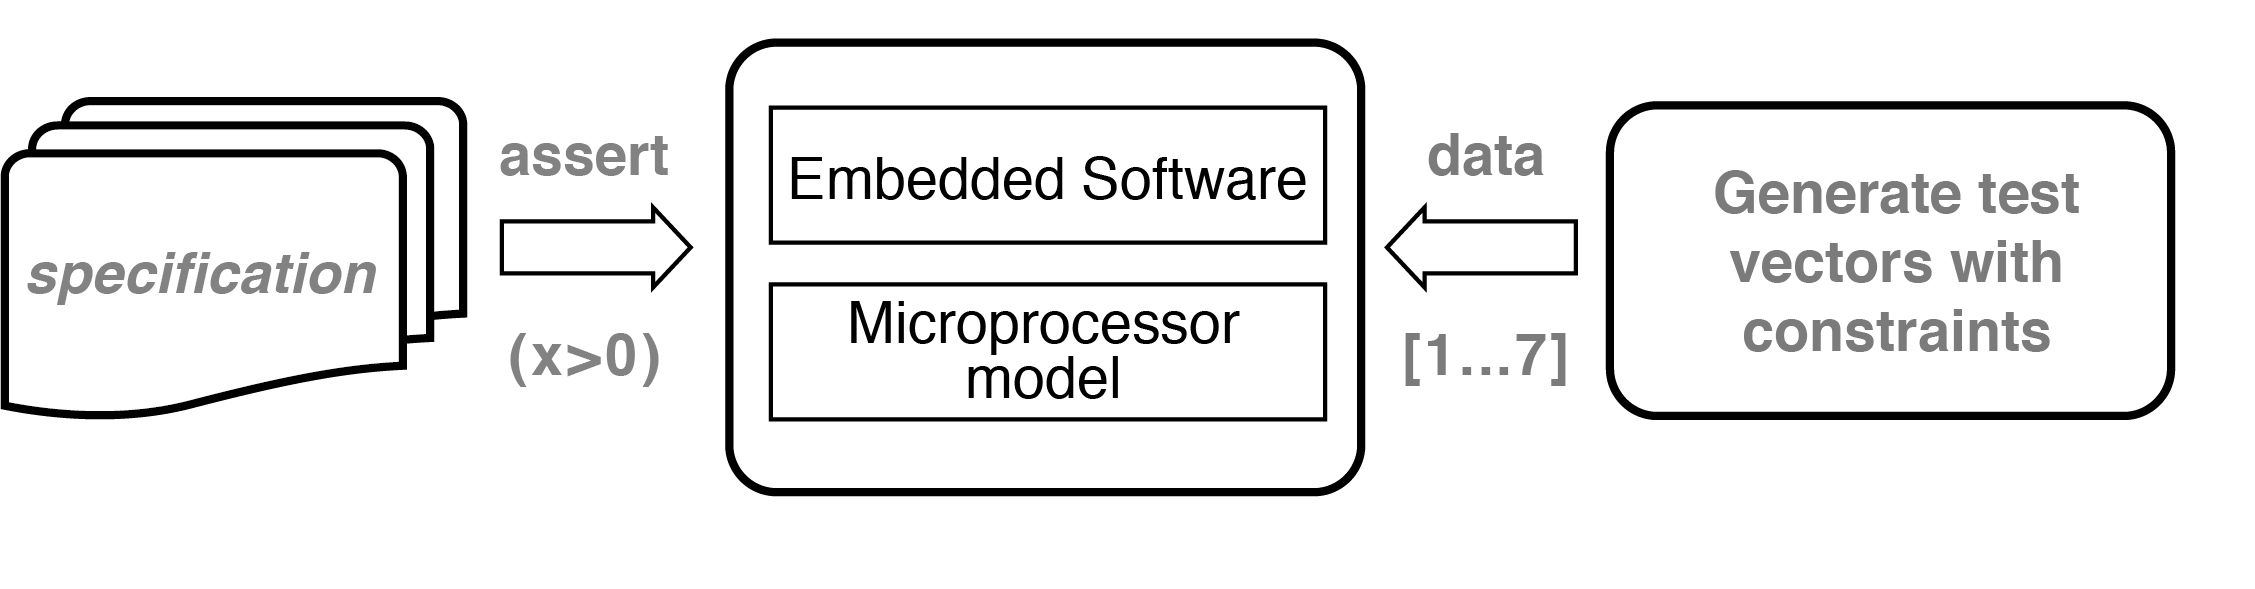
\includegraphics[width=\textwidth]{figure4.jpg}
	\caption{Verification methodologies for embedded systems.}
	\label{verification-methodologies}
\end{figure}


In particular, the main challenges regarding verification of embedded systems lie on improving coverage, where more system functions are verified, reducing verification time, {\it i.e.}, pruning state-space exploration during verification, providing completeness, {\it i.e.},  if all possible states can be reached and evaluated, and incorporating system models, which allow specific checks regarding system behavior and not only code correctness. Additionally, embedded system verification raises additional challenges, such as:
%
\begin{enumerate}
	\item Time and energy constraints;
	\item Handling of concurrent software;
	\item Platform restrictions;
	\item Verification of code pieces or modules that rely on larger structures;
	\item Legacy designs; %, which are usually developed with low-level languages.
	\item Support to different programming languages, frameworks, and interfaces;
	\item Correct code instrumentation;
	\item Handling of non-linear and non-convex optimization problems;
	\item Incorporation of new and adapted checks, due to system or environment evolution.
\end{enumerate}

Indeed, the first two aspects are of extreme relevance in micro-grids and cyber-physical systems, in order to ensure reliability, which is a key issue for (smart) cities, industries, and consumers, and the third one is essential in systems that implement device models, such as digital filters and controllers, which present a behavior that is highly dependent on signal inputs and outputs and whose deployment may be heavily affected by hardware restrictions. The fourth aspect deals with code that relies on existing infrastructures and must be compliant with those, such as Linux kernel modules. The fifth aspect, in turn, is inherent to a large number of embedded systems from  telecommunications, control systems, and medical devices, including ECPSs. In particular, software developed for those types of embedded system has been extensively tested and verified, and also optimized for efficiency over years of development. Therefore, when a new product is derived from a given platform, a lot of legacy code is usually reused for improving development time and code quality. The sixth aspect is related to evolving development processes and technologies, which may delay the application of suitable verification and synthesis approaches, if verifiers and synthesizers do not support different programming languages and interfaces. The seventh aspect highlights a subjective task in verification: where one must insert an evaluation point or assertion, in order to correct address a property. The eighth one is related to the widespread use of embedded systems in autonomous-vehicle navigation systems~\cite{Adouane16}, which demands optimization solving during their execution for a wide range of functions, including non-linear and non-convex problems using fixed- and floating-point arithmetic. The ninth aspect is a consequence of changes in environment or different applications and scenarios, which may present new problems to embedded systems that did not exist or were not tackled during their development. Such a challenge is also closely related to ML techniques, given that they may be integrated into commercial systems and have the potential to devise new and refined control strategies, which must then be identified, checked, and validated. For instance, a diagnostic system may employ techniques that make it able to learn new tumor patterns and them warn their presence on patients' bodies, but a wrong updated model may compromise earlier traditional assessments and erroneously perform new ones, which should be verified and validated. Finally, the latter also raises another question: an embedded system must be checked only when it is developed/created or also during its life cycle, in order to ensure that improved models and actions are sound and reliable? That is an issue that will probably concern researchers, when ML becomes mature and widely spread in software verification.

Those nine challenges place additional difficulties for developing reliable synthesizers for embedded systems, especially for cyber-physical systems and micro-grids, where controlled objects ({\it e.g.}, physical plants) typically exhibit continuous behavior (which may eventually change), whereas controllers (usually implemented by real-time computer systems) operate in discrete time and over a quantized domain. In particular, synthesizers for those systems need to consider the effects of quantizers (A/D and D/A converters), when a digital equivalent of the controlled object is considered, {\it i.e.}, a model of their physical environment (cf. intelligent product in Figure~\ref{intelligent-product}). Additionally,  finite-precision arithmetic and their related rounding errors need to be considered, when correct-by-construction code is generated for embedded systems.

%--------------------------------------
\section{Research Problem (RP)}
\label{Research-Problem}
%--------------------------------------

This position paper tackles seven major problems in computer-aided verification and synthesis for ECPS, which are (partially) open in current published research.

\textbf{(RP1)} provision of suitable encoding into SMT \cite{BarrettSST09}, which may extend background theories typically supported by SMT solvers, with the goal of reasoning accurately and effectively about realistic ECPS.

\textbf{(RP2)} exploitation of SMT techniques to leverage bounded model checking of multi-threaded software, in order to mitigate the state-explosion problem due to thread interleaving.
	
\textbf{(RP3)} proof of correctness and timeliness of ECPS, by taking into account stringent constraints imposed by hardware platforms.
	
\textbf{(RP4)} incorporation knowledge about system purpose and associated features, which aims to detect system-level and behavior failures.

\textbf{(RP5)} provision of tools and approaches capable of addressing different programming languages and application interfaces, with the goal of reducing the time needed to adapt current verification techniques to new developments and technologies.

\textbf{(RP6)} development of automated synthesis approaches that are algorithmically and numerically sound, in order to handle (control) software that is tightly coupled with physical environments, by considering uncertain models and FWL effects.

\textbf{(RP7)} provision of a unified framework, which is able to tackle high and low level properties, as well as system behavior, with the potential to lead to another degree of completeness, in such a way that every implementation aspect of ECPS is addressed and evaluated.

Section~\ref{achievements} outlines contributions toward such research problems.

%--------------------------------------
\section{Current Achievements and \\ Future Trends}
\label{achievements}
%--------------------------------------

\textbf{(RP1)} Cordeiro, Fischer, and Marques-Silva proposed the first SMT-based BMC for full C programs, called Efficient SMT-Based Context-Bounded Model Checker (ESBMC)~\cite{Cordeiro12}, which was later extended to support C++98 programs~\cite{ECBS13}, CUDA programs~\cite{cudalucas,Pereira17}, and Qt-based consumer electronics applications~\cite{Sousa15}. This approach was also able to find undiscovered bugs related to arithmetic overflow, buffer overflow, and invalid pointer, in standard benchmarks, which were later confirmed by the benchmarks' creators ({\it e.g.}, NOKIA, NEC, NXP, and VERISEC)~\cite{CordeiroF11,Cordeiro12}. Other SMT-based BMC approaches have also been proposed and implemented~\cite{MerzFS12}, but the coverage and verification time of all existing ones are still limited to specific program classes, especially for those that contain intensive floating-point arithmetic and dynamic memory allocation~\cite{Beyer14,BeyerSVCOMP15}. One possible research direction is to bridge the gap between BMC tools and SMT solvers, propose background theories, and develop more efficient decision procedures, in order to handle specific program classes. In this particular research direction, the European Project SC$^2$ (Satisfiability Checking and Symbolic Computation: uniting two communities to solve real problems) aims to further extend background theories supported by SMT solvers, in order to solve problems related to security and safety of computer systems (or large mathematical problems), through the development of radically improved software tools~\cite{DBLP:journals/cca/AbrahamA0BBBCDE16}.

\textbf{(RP2)} The SMT-based BMC approach proposed by Cordeiro, Fischer, and Marques-Silva was further developed to verify correct lock acquisition ordering and absence of deadlocks, data races, and atomicity violations in multi-threaded software based on POSIX and CUDA libraries~\cite{CordeiroF11,Pereira17}, considering monotonic partial-order reduction~\cite{KahlonWG09} and state-hashing techniques, in order to prune state-space exploration~\cite{morse15}. Recent advances for verifying multi-threaded C programs have been proposed to speed up verification times, which significantly prune state-space exploration~\cite{Inverso14,civl15}, and also extensions to verify the Debian GNU/Linux distribution, based on a context- and thread-sensitive abstract interpretation framework~\cite{DBLP:conf/kbse/KroeningPSW16}, were made available; however, the set of concurrent-program classes ({\it e.g.}, CUDA, OpenCL, and MPI) that can be verified is still very limited. One possible research direction is to further extend BMC of multi-threaded C programs via Lazy Sequentialization~\cite{Inverso14}, in order to analyze unsatisfiability cores~\cite{Grumberg05}, with the goal of removing redundant behaviour or analyzing interpolants~\cite{McMillan11} and then prove non-interference of context switches.

\textbf{(RP3)} Novel approaches to model check embedded software using \textit{k}-induction and invariants were proposed and evaluated in literature, which demonstrate its effectiveness in some real-life embedded-system applications~\cite{Gadelha15,Brain15,Rocha15,Donaldson10,Rocha17}; however, the main challenge remains still open, {\it i.e.}, to compute and strengthen loop invariants for proving program correctness and timeliness in a more efficient and effective way, in order to be competitive with other model-checking approaches. In particular, invariant-generation algorithms have substantially evolved over the last years, with the goal of discovering inductive invariants of programs~\cite{pips:2013,Henry:2012} or continuously refine them during verification~\cite{Beyer15}; however, there is still a lack of studies for exploiting the combination of different invariant-generation algorithms ({\it e.g.}, interval analysis, linear inequalities, polynomial equalities and inequalities) and how to strengthen them during verification, in order to ensure system robustness w.r.t. implementation aspects. Finally, optimal configurations for invariant generators are still of paramount importance, given that applications with code based on different aspects may benefit from different setups.

\textbf{(RP4)} State-of-the-art SMT-based context-BMC approaches were extended to verify overflow, limit cycle, time constraints, stability, and minimum phase, in digital systems. Indeed, digital filters and controllers~\cite{dsv_spin2015,esbmc_controller,esbmc_filter} were tackled, in order to specify system-level properties of those systems, using linear-time temporal logic~\cite{JMorse15}. In particular, a specific UAV application was tackled, with the goal of verifying its attitude controllers~\cite{Bessa16,Chaves17}. More recently, other implementation aspects were added to the existing verification framework, including magnitude, phase, poles, and zeros, which provide deeper analysis regarding digital systems, by tackling frequency-domain parameters, permissible deviation, and associated natural response \cite{sbrtdaniel}. In general, however, there is still a lack of studies to verify system-level properties related to ECPS; emphasis should be given to micro-grids~\cite{xu15}, which require high-dependability requirements for computation, control, and communication. Additionally, the application of automated fault detection, localization, and correction techniques to digital systems represents an important research direction to make BMC tools useful for ECPS engineers~\cite{Alves15}.

{\textbf{(RP5)} Although ESBMC \cite{Cordeiro12} was extended to support C/C++ and some variants, new application interfaces and programming languages are often developed, which require suitable software verification tools. Indeed, it would be interesting if a new programming language model could be loaded, which along with a BMC core could check different programs. Some work towards that was already presented by Sousa, Cordeiro, and Filho~\cite{Garcia16}, which employed operational models for checking Qt-based programs from consumer electronics. In summary, the BMC core (in that case, ESBMC) is not changed (it is still C/C++ code), but instead an operational model, which implements the behavior and features of Qt libraries, is used to provide the new code structure to be checked. This approach could adopt the clang compiler~\cite{Lopes:2014:GSL:2692607}, which is already widely used in industry~\cite{clang-usage}, in order to produce an Abstract Syntax Tree (AST) for a given programming language ({\it e.g.}, C/C++/ObjectiveC/ObjectiveC++). This AST can then be converted either to an intermediate representation (IR) of the underlying verifier or to LLVM bitcode that is already produced by clang. Obviously, a completely new language may present new structures and resources; however, if different inputs are parsed and converted into a form that preserves every aspect of their structure, that can then be analyzed and verified in an unified way. Such research problem is closely related to the first one \textbf{(RP1)} and has the potential to devise a new paradigm in software verification.

{\textbf{(RP6)} State-of-the-art synthesis approaches for embedded (control) systems typically disregard the platform in which the embedded system software operates and restrict themselves to generate code that do not take into account FWL effects. The synthesized system, however, must include the physical plant to avoid serious system's malfunctioning (or even a catastrophe), due to the embedded (control) software, {\it e.g.}, the Mars Polar Lander did not account for leg compressions prior to landing~\cite{Jackson16}. Research in this direction has made some progress to design, implement, and evaluate an automated approach for generating correct-by-construction digital controllers that is based on state-of-the-art inductive synthesis techniques~\cite{Abate17}. Nonetheless, there is still little evidence whether that approach can scale for larger systems modeled by other types of representation ({\it e.g.}, state-space). In addition to that, another research direction for synthesizers is to generate code for UAV trajectory and mission planning by taking into account system's dynamics and nonholonomic constraints~\cite{Araujo16}. As a consequence, verifiers and synthesizers need to handle a wide range of functions, including non-linear and non-convex optimization problems based on both fixed- and floating-point arithmetic.

\textbf{(RP7)} Embedded systems are typically implemented in low- and medium-level programming languages ({\it e.g.}, ANSI-C/C++/Java). Given the availability of different programming languages for writing code for ECPS, the provision of a unified framework able to tackle low- and high-level properties, as well as system behavior, is needed to achieve code coverage in real applications. The clang compiler~\cite{Lopes:2014:GSL:2692607} seems to offer a simple and strong approach to lead software verification to another degree of completeness so that every implementation aspect of an embedded system can be addressed and evaluated. In particular, by using the clang compiler as front-end for a software verification tool, we avoid the need for maintaining a proprietary front-end (a real challenge nowadays, given that the C and C++ standards are rapidly evolving), and then focus on the main objective: formal program verification. Here, we provide only operation models to tackle low- and high-level system properties via an abstract representation of the associated libraries, which conservatively approximates their semantics. The clang compiler offers an industrial quality analyzer and an application programming interface to access and traverse its internal AST, which can then be used by software verifiers to generate their IR or alternatively analyze the LLVM bitcode produced by clang. 

Lastly, yet importantly, BMC tools like CBMC~\cite{Clarke04}, ESBMC~\cite{MorseCNF13,MorseRCN014}, SMACK~\cite{Haran15}, and LLBMC~\cite{MerzFS12} represent the most prominent approaches for verifying C programs, as observed in the Intl. Competition on Software Verification~\cite{Beyer14,BeyerSVCOMP15,Beyer16}, where verifiable (correctness and violation) witnesses are of extreme importance for evaluating software verifiers~\cite{BeyerW15,RochaIFM12}. The increasing number of verification tasks being added every year to this competition allows developers to further improve their verifiers by implementing new types of abstraction and simplification techniques. As a consequence, the continuous development and improvement of verifiers can leverage more efficient synthesizers and further increase the reliability of verified ECPS.

%----------------------------------------------------------------------------
\section{New Applications: Beyond Code Correctness}
\label{Newapp}
%----------------------------------------------------------------------------

As already mentioned in section \ref{sec:model}, problems that are not directly related to code correctness may be tackled with formal methods, as long as they are conveniently modeled. Ara\'ujo {\it et al.} \cite{Araujo16} employed SMT for handling non-convex optimization problems, with the goal of ensuring optimal solutions. Indeed, it is possible to recursively re-constrains a model checking procedure, by using the current counterexample as a seed for the next run, until a global minimum is achieved. Nonetheless, elapsed execution times are still a bottleneck for some applications, such as changes in UAV trajectories, but that can be improved, through the use of simplification techniques and problem constraints.

In the same fashion, other problems may benefit from the recursive-refinement approach provided by SMT-based verification schemes. For instance, de Jesus {\it et. al} \cite{antennasbrt} developed a simplified methodology for antenna alignment that makes use of many modules already available in satellite TV receivers, along with a suitable structure for performing position correction. In summary, a reference signal is evaluated, until an (approximately) error-free reception is acquired, which can be measured through a simple transport stream (TS) error-indication interface and further refined with other parameters, such as carrier-to-noise ratio and signal level. This way, by using an SMT-based verification method, one may map the TS error indication and other performance figures as properties and then recursively perform realignment procedures, until a counterexample is not output. It is worth noticing that associated timing requirements are more relaxed than what was mentioned in the work developed by Ara\'ujo {\it et al.}~\cite{Araujo16}, which can be seen as an advantage for such an implementation.

Regarding behavior correctness, many other applications can be tackled, such as the ones related to automatic classification. Amoedo {\it et al.} \cite{amoedo} proposed a modulation classification methodology, with the goal of spectrum sensing for opportunistic transmissions. Besides a correct software implementation, {\it i.e.}, source code, which is already covered by formal methods already available in literature \cite{esbmc_filter,Cordeiro12,Clarke04}, one may argue if the proposed methodology is able to recognize modulations under some reception condition, such as severe analog interference. This way, it would be interesting to develop a verification module for transmission and reception software, which could be capable of creating inputs related to sampled radio frequency signals, under a variety of conditions, and then unifying source code and behavior verification. In addition, that kind of implementation usually employs digital filters with specific parameters, which could also be tackled. Indeed, communication aspects of ECPSs could be tackled, as a module in system verification procedures.

ML techniques are already being used in the software verification area \cite{mlswverif,nguyen,bridge,babic07}. For instance, Hamel~\cite{mlswverif} proposed to induce a theory, through ML, that fits a test set for a program, in such a way that it implements the respective test set. Phuc \cite{nguyen}, in turn, applied decision tree C4.5 and multilayer perceptron to annotated programs (metrics related to structure and semantics) and tackled the generation of test sets satisfying the desired constraints. Bridge studied the automation of heuristic selection based on features, regarding first-order logic theorem proving, and Hutter {\it et. al} \cite{babic07} showed that ML can be used for improving SAT solvers regarding huge verification tasks, when applied to parameter tuning~\cite{babic07}. Seshia {\it et al.}~\cite{Seshia17}, in turn, showed that control syntheses based on ML is also a trend, since it has been applied to different applications and model classes~\cite{Jha10,Sadigh14}. Finally, ML can also be used for invariant computation and strengthening, which is a major bottleneck in \textit{k}-induction verification based on invariant algorithms. As a consequence of what was presented, it seems worthwhile to pursue integration of ML into BMC-based checkers, given that it has the potential to tackle many open problems or at least enhance existing solutions. 

%--------------------------------------
\section{Conclusions}
\label{conclusions}
%--------------------------------------

This paper presented the main challenges related to the verification of design correctness, in ECPS, and also raised some important side considerations about synthesis. In particular, it emphasizes that stringent constraints imposed by the underlying hardware ({\it e.g.}, real-time, memory allocation, interrupts, and concurrency), along with system behavior models, must be considered during verification and synthesis. Additionally, there is little evidence that model checking ECPS using \textit{k}-induction (and invariants), which extends BMC-based approaches from falsification to verification, can be applied to formally verify correctness and timeliness of ECPS. 

Given that software complexity has significantly increased in ECPS, there are still some (recent) advances to stress and exhaustively cover the system state space, in order to verify low-level properties that have to meet the application's deadline, access memory regions, handle concurrency, and control hardware registers. There is a trend towards incorporating knowledge about the system to be verified, which may take software verification and synthesis one step further, where not only code correctness will be addressed, but also full system reliability. In addition, it seems interesting to provide behavioral models when new application interfaces or programming language features are used, in order to extend capabilities of current verification tools, without changing the core BMC module. Finally, there are some bottlenecks in software verification that are possible to be handled with machine learning, given some initial studies carried out in the current literature, which may represent another step towards a unified and complete approach that combines code verification, behavior correctness, environment adaptation, and system evolution.

As future work, the main goal of this research is to extend BMC as a design, verification, and synthesis tool for achieving correct-by-construction ECPS implementations. Special attention will be given to modern micro-grids, considering small-scale versions of a distributed system, so that reliability and other system-level properties ({\it e.g.}, carbon emission reduction in smart cities) are amenable to automated verification and synthesis, probably through behavior models. Additionally, ML techniques will be incorporated to BMC frameworks, in order to provide flexibility and specific-problem tuning.

\bibliographystyle{ACM-Reference-Format}
\bibliography{refs}


% conference papers do not normally have an appendix


% use section* for acknowledgment
%\section*{Acknowledgment}

%The authors would like to thank...
%The authors thank M. Dangl for reviewing a draft version of this paper.~This research was supported by CNPq $475647$/$2013$-$0$ grant.



%\begin{thebibliography}{1}

%1
%\bibitem{Kopetz11}
%H.~Kopetz:
%\newblock {\em {Real-Time Systems - Design Principles for Distributed Embedded Applications}}.
%\newblock Real-Time Systems Series, Springer, ISBN 978-1-4419-8236-0, pp. 1--376, 2011.
%
%%2
%\bibitem{xu15}
%Xua X., Jiaa H., Wanga D., Yub D., Chiangc H.:
%\newblock {\em {Hierarchical energy management system for multi-source multi-product microgrids}}.
%\newblock In: Renewable Energy, v. 78, pp. 621--630, 2015.
%
%%3
%\bibitem{leeCPS}
%Lee E.:
%\newblock {\em {Cyber-physical Systems: Design Challenges}}.
%\newblock In: International Symposium on Object Oriented Real-Time Distributed Computing, pp. 363--369, 2008.
%
%%4
%\bibitem{leeCPS2}
%Lee E.:
%\newblock {\em {The Past, Present and Future of Cyber-Physical Systems: A Focus on Models}}. 
%\newblock In: Sensors 15(3): pp. 4837--4869, 2015.
%
%%5
%\bibitem{groza2015formal}
%Groza A., Letia I., Goron A., Zaporojan S.: 
%\newblock {\em {A formal approach for identifying assurance deficits in unmanned aerial vehicle software}}.
%\newblock In: Progress in Systems Engineering, Springer, pp. 233--239, 2015.
%
%%6
%\bibitem{Cordeiro09}
%Cordeiro L., Fischer B., Chen H., Marques-Silva J.:
%\newblock {\em {Semiformal Verification of Embedded Software in Medical Devices Considering Stringent Hardware Constraints}}.
%\newblock In: International Conference on Embedded Software and Systems, pp. 396--403, 2009.
%
%%7
%\bibitem{munir}
%Munir S., Stankovic J. A., Liang C.-J. M., Lin S.:
%\newblock {\em {Cyber Physical System Challenges for Human-in-the-Loop Control}}. 
%\newblock In: 8th International Workshop on Feedback Computing, pp. 1--4, 2013.
%
%%8
%\bibitem{Abate17}
%Abate A., Bessa I., Cattaruzza D., Cordeiro L., David C., Kesseli P., Kroening D.:
%\newblock {\em {Sound and Automated Synthesis of Digital Stabilizing Controllers for Continuous Plants}}.
%\newblock In: 20th ACM International Conference on Hybrid Systems: Computation and Control, 2017 (to appear).
%
%%9
%\bibitem{ldd}
%Witkowski T., Blanc N., Kroening D., Weissenbacher G.:
%\newblock {\em {Model checking concurrent linux device drivers}}.
%\newblock In: 22nd IEEE/ACM international conference on Automated software engineering, pp. 501--504, 2007.
%
%%10
%\bibitem{mlembe}
%S.~Virtanen:
%\newblock {\em {Advancing Embedded Systems and Real-Time Communications with Emerging Technologies}}.
%\newblock IGI Global, ISBN 978-1466660342, pp. 1--502, 2014.
%
%%11
%\bibitem{Kroening15}
%Kroening D., Liang L., Melham T., Schrammel P., Tautschnig M.:
%\newblock {\em {Effective Verification of Low-Level Software with Nested Interrupts}}. 
%\newblock In: Design, Automation and Test in Europe, pp. 229--234, 2015.
%
%%12
%\bibitem{cudalucas}
%Monteiro F. R., da Silva Alves E. H., Silva I. S., Ismail H., Cordeiro L. C., de Lima Filho E. B.:
%\newblock {\em {ESBMC-GPU A Context-Bounded Model Checking Tool to Verify CUDA Programs}}. 
%\newblock In: Science of Computer Programming xx(y): pp. xxxx--xxxx, 2017.
%
%%13
%\bibitem{stochmodel}
%Bargmann H.:
%\newblock {\em {The role of stochastic modelling in engineering science}}.
%\newblock In: Acta Mecanica 125(1), pp. 63--71, 1997.
%
%%14
%\bibitem{Shoukry}
%Shoukry Y., Nuzzo P., Puggelli A., Sangiovanni-Vincentelli A. L., Seshia S. A., Tabuada P.:
%\newblock {\em {Secure State Estimation for Cyber Physical Systems Under Sensor Attacks: A Satisfiability Modulo Theory Approach}}.
%\newblock {IEEE} Trans. Automatic Control PP(99), pp. 1--16, 2017.
%
%%15
%\bibitem{cpsattack}
%Liu Y., Ning P., Reiter M. K.:
%\newblock {\em {“False data injection attacks against state estimation in electric power grid}}.
%\newblock In: ACM Conference on Computer and Communications Security, pp. 21--32, 2009.
%
%%16
%\bibitem{Araujo16}
%Araujo, R., Bessa, I., Cordeiro, L., Chaves Filho, J.:
%\newblock {\em{ SMT-based Verification Applied to Non-convex Optimization Problems}}. 
%\newblock In: VI Brazilian Symposium on Computing Systems Engineering, 2016 (to appear).
%
%%17
%\bibitem{Biere99}
%Biere A., Cimatti A., Clarke E., Zhu Y.:
%\newblock {\em {Symbolic Model Checking without BDDs}}. 
%\newblock In: Tools and Algorithms for Construction and Analysis of Systems, LNCS 1579, pp. 193--207, 1999.
%
%%18
%\bibitem{handbook09}
%Biere A., Heule M., van Maaren H., Walsh T., eds.:
%\newblock {\em {Handbook of Satisfiability}}.
%\newblock Volume 185 of Frontiers in Artificial Intelligence and Applications., {IOS} Press, 2009.
%
%%19
%\bibitem{BarrettSST09}
%Barrett C., Sebastiani R., Seshia S.A., Tinelli C.:
%\newblock {\em {Satisfiability Modulo Theories}}. 
%\newblock In: Volume 185 of Frontiers in Artificial Intelligence and Applications. IOS Press, pp. 825--885, 2009.
%
%%20
%\bibitem{Armando2009}
%Armando A., Mantovani J., Platania L.:
%\newblock {\em {Bounded Model Checking of Software Using SMT Solvers Instead of SAT Solvers}}. 
%\newblock In: {SPIN} Workshop on Model Checking Software, LNCS 3925, pp. 146-162, 2006.
%
%%21
%\bibitem{Bradley07}
%Bradley A., Manna Z.:
%\newblock {\em {The calculus of computation - decision procedures with applications to verification}}. 
%\newblock In: Springer, pp. I-XV, pp. 1--366, 2007.
%
%%22
%\bibitem{Thomas01}
%Thomas Ball and Sriram~K. Rajamani.
%\newblock {\em SLIC: A Specification Language for Interface Checking (of C)}.
%\newblock Technical Report MSR-TR-2001-21, Microsoft Research, 2001.
%
%%23
%\bibitem{Strichman08}
%Daniel Kroening and Ofer Strichman.
%\newblock {\em Decision Procedures: An Algorithmic Point of View}.
%\newblock Springer Publishing Company, Incorporated, 2008.
%
%%24
%\bibitem{Appel97}
%Andrew~W. Appel.
%\newblock {\em Modern Compiler Implementation in C: Basic Techniques}.
%\newblock Cambridge University Press, New York, NY, USA, 1997.
%
%%25
%\bibitem{Tseitin83}
%G.~S. Tseitin.
%\newblock On the complexity of derivation in propositional calculus.
%\newblock In {\em In J. Siekmann and G. Wrightson, editors, Automation of
%  Reasoning 2: Classical Papers on Computational Logic 1967-1970}.
% 
% %26
% \bibitem{PatarinG97}
%Jacques Patarin and Louis Goubin.
%\newblock Trapdoor one-way permutations and multivariate polynominals.
%\newblock In {\em ICICS}, {\em LNCS} 1334, pages 356--368. Springer, 1997. 
%
%%27
%\bibitem{Clarke04}
%Clarke E., Kroening D., Lerda F.:
%\newblock {\em {A Tool for Checking {ANSI-C} Programs}}.
%\newblock In: Tools and Algorithms for the Construction and Analysis of Systems. LNCS 2988, Springer Berlin Heidelberg, pp. 168--176, 2004.
%
%%28
%\bibitem{MerzFS12}
%Merz F., Falke S., Sinz C.:
%\newblock {\em {{LLBMC}: Bounded Model Checking of {C} and {C++} Programs using a Compiler {IR}}}.
%\newblock In: International Conference on Verified Software: Theories, Tools, Experiments. LNCS 7152, pp. 146--161, 2012.
%
%%29
%\bibitem{CordeiroF11}
%Cordeiro L., Fischer B.:
%\newblock {\em {Verifying Multi-threaded Software using {SMT}-based Context-Bounded Model Checking}}.
%\newblock In: International Conference on Software Engineering. pp. 331--340, 2011.
%
%%30
%\bibitem{Ivancic05}
%Ivanicic F., Shlyakhter I., Gupta A., Ganai, M.K.:
%\newblock {\em {Model Checking {C} Programs using {F-Soft}}}.
%\newblock In: International Conference on Computer Design: VLSI in Computers and Processors, pp. 297--308, 2005.
%
%%31
%\bibitem{Cordeiro12}
%Cordeiro L., Fischer B., Marques{-}Silva J.:
%\newblock {\em {{SMT}-based Bounded Model Checking for Embedded {ANSI-C} Software}}.
%\newblock {IEEE} Trans. Software Eng. 38(4), pp. 957--974, 2012.
%
%%32
%\bibitem{EenS03}
%E{\'{e}}n, N., S{\"{o}}rensson, N.:
%\newblock {\em {Temporal Induction by Incremental {SAT} Solving}}.
%\newblock Electronic Notes in Theoretical Computer Science 89(4), pp. 543 -- 560, 2003.
%
%%33
%\bibitem{Sheera00}
%Sheeran M., Singh S., St{\aa}lmarck G.:
%\newblock {\em {Checking Safety Properties using Induction and a {SAT}-solver}}.
%\newblock In: International Conference on Formal Methods in Computer-Aided Design. Springer-Verlag, pp. 108--125, 2000.
%
%%34
%\bibitem{4610935}
%{IEEE} standard for floating-point arithmetic.
%\newblock {\em IEEE Std 754-2008}, pages 1--70, Aug 2008.
%
%%35
%\bibitem{Goldberg91whatevery}
%David Goldberg.
%\newblock What every computer scientist should know about floating point
%  arithmetic.
%\newblock {\em ACM Computing Surveys}, 23(1):5--48, 1991.
%
%%36
%\bibitem{pips:2013}
%ParisTech M.:
%\newblock {\em {PIPS: Automatic Parallelizer and Code Transformation Framework}}. 
%\newblock Accessed 21 February 2016
%
%%37
%\bibitem{Henry:2012}
%Henry J., Monniaux D., Moy M.: 
%\newblock {\em {PAGAI: A Path Sensitive Static Analyser}}. 
%\newblock In: Electronic Notes in Theoretical Computer Science, pp. 15--25, 2012.
%
%%38
%\bibitem{Beyer15}
%Beyer D., Dangl M., Wendler P.:
%\newblock {\em {Boosting \textit{k}-Induction with Continuously-Refined Invariants}}.
%\newblock In: International Conference on Computer-Aided Verification, LNCS 9206, pp. 622--640, 2015.
%
%%39
%\bibitem{Gadelha15}
%Gadelha M., Ismail H., Cordeiro L.:
%\newblock {\em {Handling Loops in Bounded Model Checking of C Programs via \textit{k}-Induction}}.
%\newblock In: International Journal on Software Tools for Technology Transfer (to appear), 2015.
%\newblock http://dx.doi.org/10.1007/s10009-015-0407-9
%
%%40
%\bibitem{Brain15}
%Brain M., Joshi S., Kroening D., Schrammel P.:
%\newblock {\em {Safety Verification and Refutation by k-Invariants and \textit{k}-Induction}}.
%\newblock In: International Symposium on Static Analysis, LNCS 9291, pp. 145--161, 2015.
%
%%41
%\bibitem{Rocha15}
%Rocha H., Ismail H., Cordeiro L., Barreto R.:
%\newblock {\em {Model Checking Embedded C Software using \textit{k}-Induction and Invariants}}.
%\newblock In: V Brazilian Symposium on Computing Systems Engineering, pp. 90--95, 2015.
%
%%42
%\bibitem{Kinductor}
%Donaldson A., Haller L., Kroening D., R{\"{u}}mmer, P.:
%\newblock {\em {Software Verification using \textit{k}-Induction}}.
%\newblock In: International Symposium on Static Analysis. LNCS 6887, pp. 351--368, 2011.
%
%%43
%\bibitem{Rocha17}
%Rocha, W., Rocha, H., Ismail H., Cordeiro, L., Fischer, B.:
%\newblock {\em {DepthK: A \textit{k}-Induction Verifier Based on Invariant Inference for C Programs}}. 
%\newblock In: International Conference on Tools and Algorithms for the Construction and Analysis of Systems, 2017 (to appear).
%
%%44
%\bibitem{Donaldson10}
%Donaldson A., Kroening D., R{\"{u}}mmer P.:
%\newblock {\em {{SCRATCH}: A Tool for Automatic Analysis of {DMA} Races}}.
%\newblock In: ACM Symposium on Principles and Practice of Parallel Programming. ACM, pp. 311--312, 2011.
%
%%45
%\bibitem{GrosseLD09}
%Gro{\ss}e D., Le H., Drechsler R.:
%\newblock {\em {Induction-based Formal Verification of {SystemC TLM} Designs}}.
%\newblock In: International Workshop on Microprocessor Test and Verification, pp. 101--106, 2009.
%
%%46
%\bibitem{David15}
%C.~David, D.~Kroening, and M.~Lewis.
%\newblock {\em {Using program synthesis for program analysis}}.
%\newblock In: Logic for Programming, Artificial Intelligence, and Reasoning, LNCS 9450, pp. 483--498, 2015.
%
%%47
%\bibitem{Alur13}
%Alur R., Bod\'{\i}k R., Juniwal G., Martin M., Raghothaman M., Seshia S., Singh R., Solar-Lezama A., Torlak E., Udupa A.:
%\newblock {\em {Syntax-guided synthesis}}. 
%\newblock In: Formal Methods in Computer-Aided Design, pp. 1--8, 2013.
%
%%48
%\bibitem{sketch}
%A.~Solar-Lezama.
%\newblock {\em {Program sketching}}.
%\newblock In: International Journal on Software Tools for Technology Transfer, 15(5-6):475--495, 2013.
%
%%49
%\bibitem{Sharma14}
%R.~Sharma and A.~Aiken.
%\newblock {\em {From invariant checking to invariant inference using randomized search}}.
%\newblock In: Computer Aided Verification, LNCS 8559, pp. 88--105, 2014.
%
%%50
%\bibitem{dsv_spin2015}
%Ismail H., Bessa I., Cordeiro L., Lima Filho E., Chaves Filho J.:
%\newblock {\em {DSVerifier: A Bounded Model Checking Tool for Digital Systems}}. 
%\newblock In: International SPIN Symposium on Model Checking of Software, LNCS 9232, pp. 126--131, 2015.
%
%%51
%\bibitem{Monteiro16}
%F.~Monteiro:
%\newblock {\em {Bounded model checking of state-space digital systems: the impact of finite word-length effects on the implementation of fixed-point digital controllers based on state-space modeling}}. 
%\newblock In: 24th {ACM} {SIGSOFT} International Symposium on Foundations of Software Engineering, pp. 1151--1153, 2016.
%
%%52
%\bibitem{Bessa17}
%Bessa, I., Ismail, H., Palhares, R., Cordeiro, L., Chaves Filho, J.:
%\newblock {\em {Formal Non-Fragile Stability Verification of Digital Control Systems with Uncertainty}}. 
%\newblock In: IEEE Transactions on Computers, 2017 (to appear).
%
%%53
%\bibitem{selfcar}
%Fairley P.:
%\newblock {\em {Self-Driving Cars Have a Bicycle Problem}}.
%\newblock http://spectrum.ieee.org/transportation/self-driving/selfdriving-cars-have-a-bicycle-problem.
%
%%54
%\bibitem{BMCml}
%L.~Bortolussi, D. Milios, G, Sanguinetti.:
%\newblock {\em {Smoothed model checking for uncertain Continuous-Time Markov Chains}}.
%\newblock In:. Information and Computation, 2016.
%
%%55
%\bibitem{Behrend15}
%Behrend J., Lettnin D., Gruenhage A., Ruf J., Kropf T., Rosenstiel W.:
%\newblock {\em {Scalable and Optimized Hybrid Verification of Embedded Software}}. 
%\newblock In: J. Electronic Testing 31(2): pp. 151--166, 2015.
%
%%56
%\bibitem{Lettnin09}
%Lettnin D., Nalla P. K., Behrend J., Ruf J., Gerlach J., Kropf T., Rosenstiel W., Sch{\"o}nknecht V., Reitemeyer S.:
%\newblock {\em {Semiformal Verification of Temporal Properties in Automotive Hardware Dependent Software}}. 
%\newblock In: Design, Automation and Test in Europe, pp. 1214--1217, 2009.
%
%%57
%\bibitem{Adouane16}
%Vilca J., Adouane L., Mezouar Y.:
%\newblock {\em {Optimal Multi-Criteria Waypoint Selection for Autonomous Vehicle Navigation in Structured Environment}}. 
%\newblock In: Journal of Intelligent and Robotic Systems 82(2): pp. 301--324, 2016.
%
%%58
%\bibitem{ECBS13}
%Ramalho M., Lopes M., Sousa F., Marques H., Cordeiro L., Fischer B.:
%\newblock {\em {SMT-Based Bounded Model Checking of C++ Programs} }.
%\newblock In: International Conference on Engineering of Computer-Based Systems, pp. 147--156, 2013.
%
%%59
%\bibitem{Pereira15}
%Pereira P.  Albuquerque H., Marques H., Silva I., Carvalho C., Santos V., Ferreira R., Cordeiro L.: 
%\newblock {\em {Verifying CUDA Programs using SMT-Based Context-Bounded Model Checking}}.
%\newblock In: ACM Symposium on Applied Computing, Software Verification and Testing Track, pp. 1648-1653, 2016. 
%
%%60
%\bibitem{Sousa15}
%Sousa F., Cordeiro L., Lima Filho E.: 
%\newblock {\em { Bounded Model Checking of C++ Programs Based on the Qt Framework.}} 
%\newblock In: Global Conference on Consumer Electronics, pp. 179--180, 2015.
%
%%61
%\bibitem{Beyer14}
%D.~Beyer 
%\newblock {\em {Status report on software verification - (competition summary {SV-COMP})}}. 
%\newblock In: Tools and Algorithms for the Construction and Analysis of Systems, LNCS 8413, pp. 373--388, 2014.
% 
%%62
%\bibitem{BeyerSVCOMP15}
%D.~Beyer:
%\newblock {\em {Software Verification and Verifiable Witnesses - (Report on SV-COMP 2015).}} 
%\newblock In: Tools and Algorithms for the Construction and Analysis of Systems, LNCS 9035, pp. 401-416, 2015.
%
%%63
%\bibitem{KahlonWG09}
%Kahlon V., Wang C., Gupta A.:
%\newblock {\em{Monotonic Partial Order Reduction: An Optimal Symbolic Partial Order Reduction Technique}}.
%\newblock In: International Conference on Computer-Aided Verification, LNCS 5643, pp. 398--413, 2009.
%
%%64
%\bibitem{morse15}
%J.~Morse.
%\newblock {\em {Expressive and Efficient Bounded Model Checking of Concurrent Software}}.
%\newblock {University of Southampton, PhD Thesis}, 2015.
%
%%65
%\bibitem{Inverso14}
%Inverso O., Tomasco E., Fischer B., La Torre S., Parlato G.:
%\newblock {\em {Bounded Model Checking of Multi-threaded C Programs via Lazy Sequentialization.}}
%\newblock In: International Conference on Computer-Aided Verification, LNCS 8559, pp. 585-602, 2014.
%
%%66
%\bibitem{civl15}
%Zheng M, Rogers M, Luo Z, Dwyer M, Siegel S.
%\newblock {\em{{CIVL}: Formal Verification of Parallel Programs}}.
%\newblock In: International Conference on Automated Software Engineering, pp. 830--835, 2015.
%
%%67
%\bibitem{Grumberg05}
%Grumberg O., Lerda F., Strichman O., Theobald M.:
%\newblock {\em { Proof-guided underapproximation-widening for multi-process systems.}} 
%\newblock In: Symposium on Principles of Programming Languages, pp. 122--131, 2005.
%
%%68
%\bibitem{McMillan11}
%K.~McMillan:
%\newblock {\em {Widening and Interpolation.}} 
%\newblock In: International Symposium on Static Analysis, LCNS 6887, pp. 1, 2011.
%
%%69
%\bibitem{esbmc_controller}
%Bessa I., Abreu R., Cordeiro L., Filho J.:
%\newblock {\em {SMT-Based Bounded Model Checking of Fixed-Point Digital Controllers}.}
%\newblock In: Annual Conference of the Industrial Electronics Society, pp. 295--301, 2014.
%
%%70
%\bibitem{esbmc_filter}
%Abreu R., Cordeiro L., Filho E.:
%\newblock {\em {Verifying Fixed-Point Digital Filters using SMT-Based Bounded Model Checking}.}
%\newblock In: XXXI Brazilian Symposium on Telecommunications, 2013.
%\newblock http://dx.doi.org/10.14209/sbrt.2013.57
%
%%71
%\bibitem{JMorse15}
%Morse J., Cordeiro L., Nicole D., Fischer B.:
%\newblock {\em {Model Checking LTL Properties over ANSI-C Programs with Bounded Traces.}} 
%\newblock In: Software and System Modeling 14(1): pp. 65--81, 2015.
%
%%72
%\bibitem{Bessa16}
%Bessa I., Ismail H., Cordeiro L., Chaves Filho J.:
%\newblock {\em { Verification of Fixed-Point Digital Controllers Using Direct and Delta Forms Realizations.}} 
%\newblock In: Design Automation for Embedded Systems 20(2): pp. 95--126, 2016.
%
%%73
%\bibitem{Chaves17}
%Chaves L., Bessa I., Cordeiro L.:
%\newblock {\em { DSValidator: An Automated Counterexample Reproducibility Tool for Digital Systems}}. 
%\newblock In: CoRR abs/1610.07066, 2016.
%
%%74
%\bibitem{sbrtdaniel}
%de Mello D. P. M., de Freitas M. L., Cordeiro L., da Silva J\'unior W. S., de Bessa I. V., de Lima Filho E. B, Clavier L.:
%\newblock {\em{Verification of Magnitude and Phase Responses in Fixed-Point Digital Filters}}. 
%\newblock To appear in: Brazilian Symposium on Telecommunications and Signal Processing, pp. 1-5, 2017.
%
%%75
%\bibitem{Alves15}
%Alves E. , Cordeiro L., Lima Filho E.:
%\newblock {\em{ Fault Localization in Multi-Threaded C Programs using Bounded Model Checking}}. 
%\newblock In: Brazilian Symposium on Computing Systems Engineering, pp. 96-101, 2015.
%
%%76
%\bibitem{Garcia16}
%Garcia M. , Sousa F., Cordeiro, L., Lima Filho E.: 
%\newblock {\em{ ESBMC$^{QtOM}$: A Bounded Model Checking Tool to Verify Qt Applications}}. 
%\newblock In: International SPIN symposium on Model Checking of Software (to appear), 2016.
%
%%77
%\bibitem{Lopes:2014:GSL:2692607}
%Bruno~Cardoso Lopes and Rafael Auler.
%\newblock {\em Getting Started with LLVM Core Libraries}.
%\newblock Packt Publishing, 2014.
%
%%78
% \bibitem{clang-usage}
%Cade Metz.
%\newblock Why {A}pple?s swift language will instantly remake computer
%  programming, 204.
%\newblock http://www.wired.com/2014/07/apple-swift/.
%
%%79
%\bibitem{Jackson16}
%Jackson D., Vaziri M.:
%\newblock {\em{ Correct or usable? the limits of traditional verification (impact paper award)}}. 
%\newblock In: ESEC/SIGSOFT Foundations of Software Engineering, pp. 11, 2016.
%
%%80
%\bibitem{MorseCNF13}
%Morse J., Cordeiro L., Nicole D., Fischer B.:
%\newblock {\em {Handling unbounded loops with {ESBMC} 1.20}}.
%\newblock In: Tools and Algorithms for the Construction and Analysis of
%  Systems. LNCS 7795, Springer Berlin Heidelberg, pp. 619--622, 2013.
%
%%81
%\bibitem{MorseRCN014}
%Morse J., Ramalho M., Cordeiro L., Nicole D., Fischer B.:
%\newblock {\em {ESBMC} 1.22.}
%\newblock In: Tools and Algorithms for the Construction and Analysis of
%  Systems. LNCS 8413, Springer Berlin Heidelberg, pp. 405--407, 2014.
%
%%82
%\bibitem{Haran15}
%Haran A., Carter M., Emmi M., Lal A., Qadeer S., Rakamaric Z.:
%\newblock {\em{ SMACK+Corral: A Modular Verifier - (Competition Contribution)}}. 
%\newblock In: 21st International Conference Tools and Algorithms for the Construction and Analysis of Systems, LNCS 9035, pp. 451--454, 2015.
%
%%83
%\bibitem{Beyer16}
%Beyer, D.:
%\newblock {\em{ Reliable and Reproducible Competition Results with BenchExec and Witnesses (Report on SV-COMP 2016)}}. 
%\newblock In: 22nd International Conference Tools and Algorithms for the Construction and Analysis of Systems, LNCS 9636, pp. 887--904, 2016.
%
%%84
%\bibitem{BeyerW15}
%Beyer D., Dangl M., Dietsch D., Heizmann M., Stahlbauer A.:
%\newblock {\em{ Witness validation and stepwise testification across software verifiers}}. 
%\newblock In: ESEC/SIGSOFT Foundations of Software Engineering, pp. 721--733, 2015.
%
%%85
%\bibitem{RochaIFM12}
%Rocha H., Barreto R., Cordeiro L., Dias Neto A.:
%\newblock {\em{ Understanding Programming Bugs in ANSI-C Software Using Bounded Model Checking Counter-Examples}}. 
%\newblock In: International Conference on Integrated Formal Methods, LNCS 7321, pp. 128-142, 2012.
%
%%86
%\bibitem{antennasbrt}
%de Jesus A. S., rodrigues R. N., Ferreira A. N. G., Valente V. H., de Melo W. C., de Lima Filho E. B, da Silva J\'unior W. S.:
%\newblock {\em{Automatic Antenna Alignment System for Satellite Receivers Operating in C and Ku Bands}}. 
%\newblock To appear in: Brazilian Symposium on Telecommunications and Signal Processing, pp. 1-5, 2017. (in Portuguese)
%
%%87
%\bibitem{amoedo}
%Amoedo D. A., da Silva J\'unior W. S., de Lima Filho E. A.:
%\newblock {\em{Parameter Selection for SVM in Automatic Modulation Classification of Analog and Digital Signals}}. 
%\newblock In: International Telecommunications Symposium (ITS), pp. 1-5, 2014.
%
%%88
%\bibitem{mlswverif}
%Hamel L.:
%\newblock {\em {On the Use of Machine Learning in Formal Software Verification.}} 
%\newblock {Technical Report TR03-294, Dept. of Computer Science and Statistics, University of Rhode Island}, 2003.
%
%
%%89
%\bibitem{nguyen}
%Phuc N. V.,:
%\newblock {\em {The Application of Machine Learning Methods in Software Verification and Validation.}} 
%\newblock {University of Texas at Austin, master of science dissertation}, 2010.
%
%%90
%\bibitem{bridge}
%Bridge J. P.:
%\newblock {\em {Machine learning and automated theorem proving.}} 
%\newblock {Technical Report 792, Computer Laboratory, University of Cambridge}, 2010.
%
% 
% %91
%\bibitem{babic07}
%Hutter F., Babic D., Hoos H. H., Hu A. J.              
%\newblock {\em{Boosting Verification by Automatic Tuning of Decision Procedures.}}
%\newblock {In 7th International Conference Formal Methods in Computer-Aided Design {(FMCAD)}, pp. 27--34, 2007.}

%\end{thebibliography}




% that's all folks
\end{document}


